\chapter{Bundlefly:一种适合使用多芯光纤的大规模高性能互连网络低直径拓扑结构设计}
系统的实际部署实是系统构建的关键步骤,如何提高系统的可维护性,降低部署复杂度尤其重要。
随着规模的增加,机柜间较长的链路只能由光缆替代。
2008年提出的P级Roadrunner系统,光纤数目就达4万条\upcite{fuad}。2012 年Blue Gene/Q 系统光纤路数约330K条\upcite{fuad}。
随着BOA的技术发展,光电转换装置从传统的插拔式到可以集成在芯片上,
更近距离的靠近芯片,减少能耗开销,提高传输效率,降低芯片边缘面积的限制。
为了获得更好的系统性能,光纤的数目将要大幅增加。
2011年IBM提出的Power 775 系统就采用了片上集成光模块,每个机柜5k多个光模块,每个光模块引出12路光纤\upcite{fuad}。
IBM的Blue Gene/Q 系统采用了相同的光模块\upcite{fuad}。IBM的PERCS 系统使用的Hub 芯片也是采用了片上集成光模块,
分别引出40条光链路和7条电链路\upcite{percs}。Fujitsu公司预计推出的E 级系统采用的Tofu2模块采用了BOA技术,
每块板上引出30个端口,其中光缆20 个,电缆10个\upcite{tofu2}。
高性能计算系统已经从大部分采用电缆通信的方式逐渐变成大部分采用光缆通信的方式。随着E级计算时代的到来,对光纤的需求更加大,尤其是更多的机柜间长链路给物理部署、缆线的容错性、
可维护性等带来巨大的挑战。
多芯光纤技术(MCF)是一个降低系统物理部署复杂度并且提高系统的可维护性的好办法。

虽然现在数据中心和超算系统还没有普遍使用多芯光纤但是未来多芯光纤的使用是必然趋势,
一是多芯光纤技术已经日趋成熟,二是实际需求。
多芯光纤可以大大降低同等数目的单芯光纤,同时,可以降低系统维护的难度,提高系统链路容错性。2012年HOTI会议的keynote报告上,IBM 公司Doany教授就提出使用多芯光纤不仅可以提高通信带宽还便于管理\upcite{fuad}。

据我们所了解,本章节介绍的拓扑结构是世界上第一个使用多芯光纤搭建出性价比高的高性能互连网络拓扑结构。该拓扑叫Bundlefly,是一个新的直径为3的结构。Bundlefly可以在路由器端口数有限的情况下灵活的均衡机柜内和机柜间的端口数分配,同时,构造出直径为3 的大规模多芯光纤拓扑结构并满足机柜间的带宽需求。在本章节中,还分析了Bundlefly的结构特性和设计了匹配的路由算法,并模拟分析了Bundlefly和当前经典的拓扑结构的性能。结果显示可灵活配置的Bundlefly 结构相比大多数当前经典拓扑结构可以获得更好的性能。

\section{引言}

当前最快的高性能计算机系统都是几万个计算节点的规模,如“神威$\cdot$ 太湖之光”系统和“天河二号”。
而且,大规模高性能计算机系统即将迎来E级超级计算机时代,网络规模将达到几十万个计算节点。
那么,高性能互连网络对E级高性能计算机系统非常重要。与此同时,随着处理器性能和计算速度的发展,对路由器芯片带宽需求越来越迫切。
因此,使用光纤代替机柜间的长链路是保证给大规模高性能计算系统提供足够的带宽和保证一定的传输效率的必要条件。

传统机柜之间连线采用的是在芯片边缘插拔式的主动光纤。尽管芯片的计算和交换带宽都在增加,但是芯片的物理面积仍然受限。
采用在芯片边缘插拔式的光纤因为面积受限影响了光纤的数量。随着片上光模块的发展,光纤逐渐从芯片边缘更加靠近芯片内部。
这样不仅增加光纤的数目而且通过缩短了芯片和光模块的距离降低了能耗的开销。而且,因为光电转换铜线距离缩短,提高了信号传输效率\upcite{BOA}。
在IBM的Power 775系统中,其采用了片上光纤集线模块,每个机柜引出了5000 个光模块和60000条光纤\upcite{fuad}。
在IBM的Blue Gene/Q系统中,其也同样采用了Power 775系统中的光模块,整个系统有330000条光纤互连
\upcite{fuad}。在IBM 的PERCS 系统中,每个集成芯片提供41条光纤链路和7条电缆链路。
在网络最大规模下,整个系统有336000条光纤链路和131000条机柜间光纤链路\upcite{percs}。
日本富士通公司将要推出的E级计算机系统Post-FX10,其采用的Tofu 2互连模块就是每个板子提供20条光纤链路和10条电缆链路\upcite{tofu2}。

随着系统光纤数量的增加,不仅要考虑能耗和成本的开销还要考虑缆线物理封装的复杂度、容错性以及维护性。
因此,在机柜之间使用多芯光纤(MCF)代替传统的一捆光纤是未来高性能计算机系统和数据中心系统解决大量光纤封装、容错性以及维护性等问题的新方法\upcite{ofsoptics}\upcite{fuad}\upcite{furukawa2012}\upcite{fibercore}。多芯光纤允许多个纤芯被封装在同一个包层中。
虽然多个纤芯之间可能会互相信号干扰和导致信号衰减,但是已经有很多研究组已经提出了相关的解决方案\upcite{aflglobal}\upcite{design32}\upcite{optics}。
 相比单芯光纤,多芯光纤不仅能够提高传输线路的单位面积的集成密度,而且有效降低成本开销的同时增强了光纤的容错性和可维护性。使用多芯光纤降低了
 光纤的实际数量,不仅使得错误率下降,而且封装的复杂度也随之降低。另外,多芯光纤的灵活性也是选用多芯光纤代替一捆单芯光纤的主要原因。多芯光纤可以通过
 低损耗的扇入/扇出设备灵活的切换成多条单芯光纤。多芯光纤的使用不影响具体路由器之间的通信,并跟使用一捆单芯光纤连接路由器的情况一致。多芯光纤对下一代高性能计算机系统和数据中心系统机柜间设计起到很重要的作用,使用多芯光纤链接机柜的机制如图\ref{mcfcabinet}所示。

 \begin{figure}[t]
  \centering
    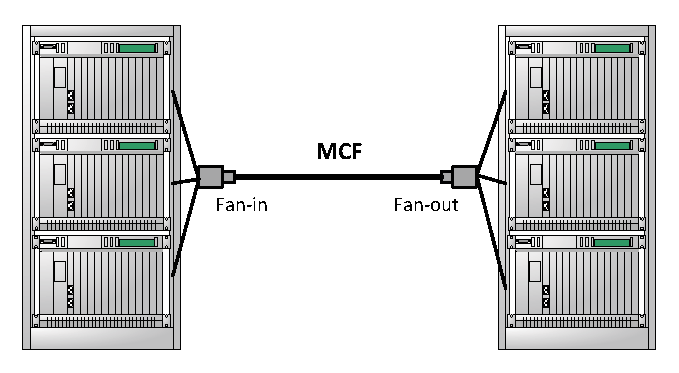
\includegraphics[width=.48\textwidth,height=.42\textwidth]{Visio-MCFcabinet.eps}
  \caption{机柜间使用多芯光纤传输原理图}
  \label{mcfcabinet}
\end{figure}

我们的目标是在尽可能使用较少端口数的路由器前提下,有效使用多芯光纤搭建性价比高的多芯光纤友好的下一代大规模高性能计算机系统。一个多芯光纤友好的网络不仅网络直径短、有较多的机柜间链路,而且即使使用当前最新的商用路由器也能构建E级计算机的规模。第二,每一个机柜都要是同构的,为了增强系统的可维护性和降低成本开销以及缆线封装的复杂度。第三,多芯光纤友好的网络结构中大多数节点对拥有两条或者两条以上的最短路径。

Dragonfly\upcite{dragonfly}是一个性价比高可扩展的高性能互连网络。但是,它不是一个多芯光纤友好的拓扑结构。
当Dragonfly的任意两个超级节点之间有$l$条链路,那么网络规模将要缩减到最大规模的$1/l$。Dragonfly最大规模时,任意两个超级节点之间只有1条链路。
一般情况下,一个超级节点是一个机柜。在实际物理布局中,虽然可以多个超级节点被封装在同一个机柜,
这样就可以在不缩小网络规模的情况下增加了机柜之间光链路数量。但是,机柜间的链路和机柜内的链路比值小于1/2。另外,Dragonfly任意两个超级节点之间只有一条链路的结构并不能很好的保证不同应用能获取较好的性能\upcite{Congestiondragonfly}。一些研究已经根据Dragonfly结构分析了不同的链路分配和任务分布的特点\upcite{Hamming}\upcite{Linkarrangements},并提出通过增加额外的机柜间链路来提高网络通信性能。但是,在Dragonfly网络上增加额外的链路会影响网络的扩展性。而且,在Dragonfly结构中,大部分节点对之间只有一条最短路径。相比Dragonfly 结构,在使用同样端口数的路由器时,直径为5的Galaxyfly 结构可以支持更大规模\upcite{Galaxyfly}。但是,在最大规模情况下任意两个超级节点之间仍然只有一条链路。虽然Galaxyfly结构扩展性优于其他拓扑结构,
但是其通过增加网络直径以支持更大规模方法限制了网络性能。随着传输速率的提升,影响网络延迟的主要因素是网络结构的直径和平均路径长度。Dragonfly
是直径为3的Galaxyfly结构。Dragonfly+\upcite{Dragonfly+}结构可以在使用同样端口数路由器下搭出Dragonfly所能构建网络的四倍规模。
但是,Dragonfly+和Drgaonfly一样,都是随着超级节点之间链路的增加,规模随之减少。Dragonfly+是一个跟Fat tree一样的间接网络。因为通信需要中继路由器,Dragonfly+ 的平均最短路径会比Dragonfly的要长。
间接网络在实际部署时不像直接网络,网络需要更多的路由器而且还区分了通信机柜和终端机柜,这在系统成本开销上和维护上都增大了难度。因此,Dragonfly+不是一个多芯光纤友好的拓扑结构。

每一个拓扑结构都不是完美的,需要在网络规模、网络直径以及机柜间链路和机柜内部链路的比值之间做一个权衡。Slim Fly\upcite{slimfly}是一个直径为2扩展性好的拓扑结构,其利用了MMS图\upcite{MMS}的技术使得较少的端口数就能支持更大的网络规模。Slim Fly在机柜间的链路与机柜内部链路的比例比Dragonfly的高,可以接近2。但是,Slim Fly的扩展性仍然受限于当前路由器端口数,比如,48端口数的Intel Omni-Path路由器\upcite{omni}已经是目前商用端口数较多的产品。而且,Slim Fly使用多芯光构造E 级规模很困难。如果使用48 端口的路由器构造网络,直径为2结构的Moore Bound\upcite{Miller05mooregraphs}上限是15K。Mellanox公司最新推出的200G Mellanox $Quantum_{TM}$路由芯片只有40个端口,160个SerDes\upcite{quantum}。 尽管这160 个SerDes可以当作80 个100G的端口来使用,但是对于直径为2结构的Moore Bound\upcite{Miller05mooregraphs}上限是69K,仍然远小于100K。而且,目前最新网络对传输速率需求已经达到200Gbps(每秒传输200G 比特位),路由器上SerDes的数量和速率发在未来几年内不会有较大的突破\upcite{Galaxyfly},这严重限制了网络拓扑结构的扩展性。另外,在Slim Fly结构中,绝大多数节点对之间只有一条最短路径。直径为2 的Galaxyfly结构跟Slim Fly 结构一样有较多的机柜间链路,但是其对路由器端口数的需求大于Slim Fly。 图\ref{constructdfv6}展示了在使用48 端口路由器条件下,直径为3和直径为2的典型拓扑结构的扩展性。FB是指三维的Flattened Butterfly 结构\upcite{Flattenedbutterfly}。图\ref{constructdfv60}中展示的是拓扑结构在任意两个机柜之间至少有一条链路的扩展性。除了Dragonfly+结构,其他拓扑结构都不能达到100K 的规模。图\ref{constructdfv61}中展示的是拓扑结构在任意两个机柜之间采用的是4 芯光纤(实际上就是机柜间至少有4 条单芯光纤)的扩展性。图中5 个拓扑结构都不能达到100K 的规模。

\begin{figure}[t]
   \begin{minipage}[t]{\textwidth}
   \centering
  \subfloat[SCF]{
    \includegraphics[width=.48\textwidth,height=.43\textwidth]{construction_difftopology_v6_0.eps}
    \label{constructdfv60}
  }
  \subfloat[MCF(l=4)]{
    \includegraphics[width=.48\textwidth,height=.43\textwidth]{construction_difftopology_v6_1.eps}
    \label{constructdfv61}
  }
  %\vspace{-.3cm}

  \caption{不同拓扑结构的扩展性}
  \label{constructdfv6}
  \end{minipage}
  \end{figure}

  因此,我们设计了一个新的多芯光纤友好的拓扑结构,Bundlefly。在使用较少端口路由器的条件下,Bundlefly权衡了路由器端口对机柜间端口数和机柜内端口数的分配并能构造更大规模的网络。Bundlefly有三个特点:第一,Bundlefly是第一个多芯光纤友好的拓扑结构,可以保证机柜间有较多的链路。第二,在端口数一定的情况,可以拥有较好的扩展性。第三,拓扑结构支持多条最短路径以达到负载均衡的作用。

  Bundlefly是一个利用了multi-star product方法构造的直径为3的拓扑结构。Bundlefly 通过减少机柜内端口数增加机柜间端口数的方式,非常适合采用多芯光纤技术封装机柜间链路。而且,Bundlefly降低了构造E级规模计算机系统对高阶路由器的要求。在Bundlefly中,多个Paley图互连成一个全局的MMS图\upcite{MMS}。 每两个相连的Paley图都是通过multi-star product方法相连。另外,Bundlefly对Paley图和multi-star product的使用保证了结构具备多条最短路径的可能。

  本章主要贡献如下:
  $\bullet$我们提出了一种新的多芯光纤友好的拓扑结构,Bundlefly。Bundlefly 利用multi-star product方法连接Paley图和MMS图。

  $\bullet$我们理论分析比较了Bundlefly和其他典型高阶互连网络。Bundlefly在使用多芯光纤的条件下展示了较高的可扩展性和较高的二分带宽以及较高的多条最短路径的比率。

   $\bullet$我们模拟评测了Bundlefly在无死锁最短路径路由和不同的非最短自适应路由算法下跟其他典型拓扑结构的性能。

   $\bullet$我们设计了一种布局模型去评测Bundlefly和其他典型拓扑结构。Bundlefly使用更多的机柜间链路可以在大部分通信模式下获得较好的性能。

\section{Bundlefly拓扑结构}

在这一章节,我们将要介绍Bundlefly的具体构造。我们首先介绍设计Bundlefly的主要思想。本章所要用到的参数将定义到表\ref{Table1}。

\begin{table}[t]
\centering
 \captionof{table}{Bundlefly参数}
  \vspace{-.3cm}
\begin{tabular}{l l}\hline
  \centering
  $N$ & Number of terminals in the network\\\hline
  $N_r$ & Number of routers in the network\\\hline
  $k$ & Router radix\\\hline
  $k'$ & The radix to other routers\\\hline
  $a$	& Number of routers in a supernode\\\hline
  $p$	& Number of terminals attached to a router\\\hline
  $h$	& Number of links to other supernodes\\
        & attached to a router\\\hline
  $q$	& Number of supernodes in a group \\
        & in Bundlefly\\\hline
  $\delta$ & $q$ $mod$ $4$\\\hline
\end{tabular}
%\vspace{-.5cm}
   \label{Table1}
   \end{table}

\subsection{构造最优化}

我们的目标是设计一个在给定路由器端口数下,不仅能够提供较高的机柜间带宽还可以在提供较好的扩展性的同时支持多条最短路径。我们定义这类拓扑结构是多芯光纤友好的拓扑结构。随着网络规模增加,构造一个大规模低延迟的网络变得困难。最著名的Moore Bound\upcite{Miller05mooregraphs}确定了在给定路由器端口数和网络直径所能构造出来的拓扑结构的最大规模上限。找到这样的理论最优值是非常困难的。而且,这样最大规模的网络任意两个节点之间往往只有一条最短路径。相反,根据给定的网络规模以及路由器端口数,找到网络直径较短结构的方法更容易。而且这类次优网络结构更加实用,尤其是路径多样性方面。一些方法可以找到这种低直径多路径的结构\upcite{MSP}。Multi-star product方法就是一种适合构造多芯光纤友好的拓扑结构方法。 采用multi-star product方法有三个主要因素:第一,我们可以使用已知的、较小的结构去构造新的大规模网络。第二,采用这种方式构造的图有严格的对称性,这可以大大降低网络在实际部署的复杂度和通信之间的开销。第三,在封装节点时,可以根据构造模块划分机柜和将多芯光纤使用在机柜间的链路上。

Multi-star product的定义如下:$V(G_{1})$和$V(G_{2})$分别是图$G_{1}$和图$G_{2}$的节点数。
对图$G_{1}$中的所有边定义一个方向,$\vec{E_{1}}$是图$G_{1}$中有向边的集合。Multi-star product实际上就是一个$\phi$函数。
图$G_{1}*_{\phi} G_{2}$就是通过multi-star product方法构造一个规模为$V(G_{1})\times V(G_{2})$的结构。
也就是,图$G_{1}$中的每一个节点都是一个超级节点,每个超级节点内部的结构是图$G_{2}$。
 每两个相连的超级节点都是是按照$\phi$函数进行相连。
 对于每一条有向链路$(u,v)\in \vec{E_{1}}$,$\phi(u,v,l)$则是一个$V(G_{2})$集合的双射,$l=0,1,...,m-1$。
 若节点$(u,v)$和节点$(w,x)$ 相邻,则要么$u=w$ 而且$(v,x)$ 是图$G_{2}$的一条边, 要么(u,w)是$\vec{E_{1}}$的边而且$x=\phi(u,w,l)(v)$。
 我们默认设置$m=1$,而且$\phi(u,v,l)$简写成$\phi$。例如,图$G_{1}*_{\phi} G_{2}$如图\ref{multistar0}所示。
 那么,$\phi$ 函数是$\phi(v)=(v+1)\ mod\ 3$。超级节点1 和超级节点3在图$G_{1}$ 中是相连的,因此,超级节点1和超级节点3之间根据函数$\phi$连接的关系如图\ref{multistar1}所示。

   \begin{figure}[t]
   \begin{minipage}[t]{\textwidth}
   \centering
   \vspace{2em}
  \subfloat[$G_{1}*_{\phi} G_{2}$]{
     \includegraphics[width=.55\textwidth,height=.38\textwidth]{Visio-multistar0.eps}
  \label{multistar0}
  }
  \subfloat[The function $\phi$]{
    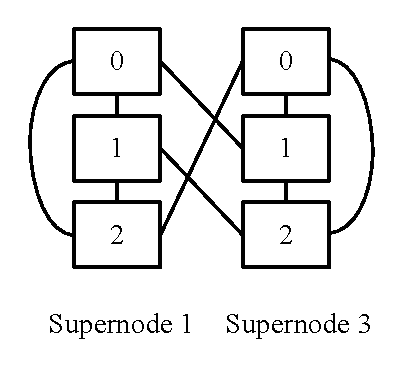
\includegraphics[width=.45\textwidth,height=.38\textwidth]{Visio-multistar1.eps}
  \label{multistar1}
  }
  \vspace{-.3cm}
  \caption{Multi-star product $G_{1}*_{\phi} G_{2}$}
  \label{multistar01}
  \end{minipage}

   \end{figure}

 \subsection{直径为3的网络结构}
   以当前路由器技术不可能构造出一个直径为2的E级规模、多芯光纤友好的拓扑结构。如果放松对网络直径的要求,我们可以容易的构造出一些扩展性好、网络直径为4的拓扑结构。例如,我们使用2维的Flattened Butterfly代替Dragonfly 超级节点内的网络,也就是说,原来超级节点内全互连结构换成了2维的Flattened Butterfly结构。任意两个超级节点之间由2维Flattened Butterfly 中的一维上的路由器进行相连。尽管构造一个直径为3的E级规模、多芯光纤友好的拓扑结构也是一件困难的事,但是,我们尝试通过multi-star product的方式按照性质\ref{diameter3}构造一个直径为3的多芯光纤友好的拓扑结构\upcite{LGGDD3}。

   \begin{prop}
\label{property1}
如果存在一个节点的置换$f$,使得$f^{2}$ 是图$G$的自同构,而且,得到的图$G*$网络直径为1,且图$G*$跟图$G$节点数一样,边涵盖图$G$的边以及图$G$置换$f$得到的边,则图$G$ 若具备性质 $P_{\ref{property1}}$。
\end{prop}

\begin{theo}
\label{diameter3}
如果$G_{1}$的网络直径为2且$G_{2}$满足性质\ref{property1},若$G_{1}*_{\phi} G_{2}$满足$x=\phi(u,w,l)(w)$的话,其中,$(u,w)$是定义图$G_{1}$的一条有向边,则$G_{1}*_{\phi} G_{2}$ 的网络直径为3。
\end{theo}

通过multi-star product的方式构造直径为3的拓扑结构关键在于如何选择合适的$G_{1}$和$G_{2}$。我们使用Paley图作为图$G_{2}$去构造更大规模的拓扑结构。因为,Paley图是一个具备性质\ref{property1}的图,而且Paley图是典型的强正则图。
在强正则图中,相邻节点和不相邻节点可能存在若干个公共邻节点。当网络节点规模大于5时,任意不相邻节点对之间存在多条最短路径。

相比较选择合适的图$G_{2}$,如何选择合适的图$G_{1}$也是非常重要和困难的。Brown's construction方法\upcite{MSP}可以构造出素数幂规模直径为2的次优规模的网络。Slim Fly 的3跳拓扑结构就是通过这种方法构造的$G_{1}$\upcite{slimfly}\upcite{LGGDD3}。但是Brown's construction方法构造的图节点的度数不唯一,除非素数幂是2的幂次方。节点度数不一致对物理封装造成困难。另外,可以通过对规模为$n$ $(n>2)$的全互连图和小规模次优图$G_{8}$采用multi-star product方法相连构造一个直径为2的拓扑结构$K_{n}*_{\phi}G_{8}$ \upcite{CLOFN}。图$G_{8}$是一个规模为8、节点度为3、直径为2的结构,具体如图\ref{multistar0}中的$G_{1}$所示。MMS图\upcite{MMS}是一个近似最优的拓扑结构。Slim Fly就是采用了这个结构作为直径为2的网络。而且,MMS图非常适合紧密的物理封装,大大减少物理封装的复杂度。在图\ref{constructdfv8}中,我们展示了一些通过multi-star product方式构造直径为3的拓扑结构,直径为3的Slim Fly(SF-3),MMS图和Paley图的组合图(MPP),Flattened Butterfly和Paley图的组合图(FBP)和$K_{n}*_{\phi}G_{8}$和Paley图的组合图(KGP)。相比较其他两个拓扑结构,MPP和SF-3展示了更好的扩展性而且可以使用48端口的路由器搭建100K规模的网络。相比较SF-3,MPP的构造和封装更加容易。因此,MPP是我们Bundlefly最好的选择。

\begin{figure}[t]
\setlength{\belowcaptionskip}{-.3cm}%
  \centering
   \begin{minipage}[t]{\textwidth}
   \centering
  \subfloat[Scalability of different topologies]{
     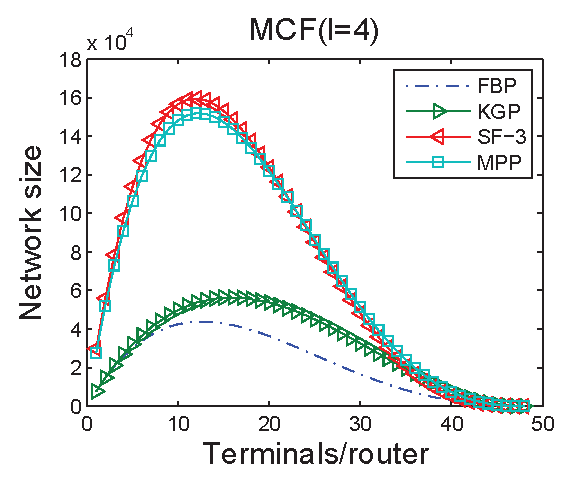
\includegraphics[width=.48\textwidth,height=.42\textwidth]{construction_difftopology_v8.eps}
  \label{constructdfv8}
  }
  \subfloat[Scalability of Bundlefly]{
    \includegraphics[width=.48\textwidth,height=.41\textwidth]{construction_difftopology_v9.eps}
  \label{constructdfv9}
  }
  \vspace{-.3cm}
  \caption{网络直径为3拓扑结构的扩展性}
  \label{constructdfv89}
  \end{minipage}
\end{figure}

 \subsection{Bundlefly的构造}

 Bundlefly是一个直径为3的层次化拓扑结构,如图\ref{mppv0}所示。Paley图作为超级节点内的结构,若干个Paley图通过multi-star product的方式连接成一个全局MMS图。每一个超级节点内$a$个路由器,如图\ref{mppv0}的超级节点所示。全局MMS图由$2\times q^2$个Paley 图构造而成,如图\ref{mppv0}中的左图所示。那么,Bundlefly内由$2\times q^2\times a$个路由器构成。$a$和$q$都是素数幂且满足$a=4w_{1}+1$和$q=4w_{2}+\delta$,其中$\delta\epsilon\{-1,0,1\}$ 和 $w_{1}, w_{2}\epsilon\mathds{N}$。 所有路由器的集合使用笛卡儿积表示: $\{0,1\}*F_{q}*F_{q}*F_{a}$。每一个路由器被一个四元组标识:$(d_{1},d_{2},d_{3},d_{4})$。$d_{1}$是MMS图中子图的编号。$d_{2}$则是MMS 图中子图的行号。$d_{3}$则是MMS图中子图的列号。$d_{4}$ 则是路由器在超级节点内的编号。每个路由器的端口数为$k=\frac{3q-\delta}{2}+\frac{a-1}{2}+p$,其中连接其他路由器的端口数为$k'=\frac{3q-\delta}{2}+\frac{a-1}{2}$。

 \begin{figure}[t]
\setlength{\belowcaptionskip}{-.5cm}
  \centering
    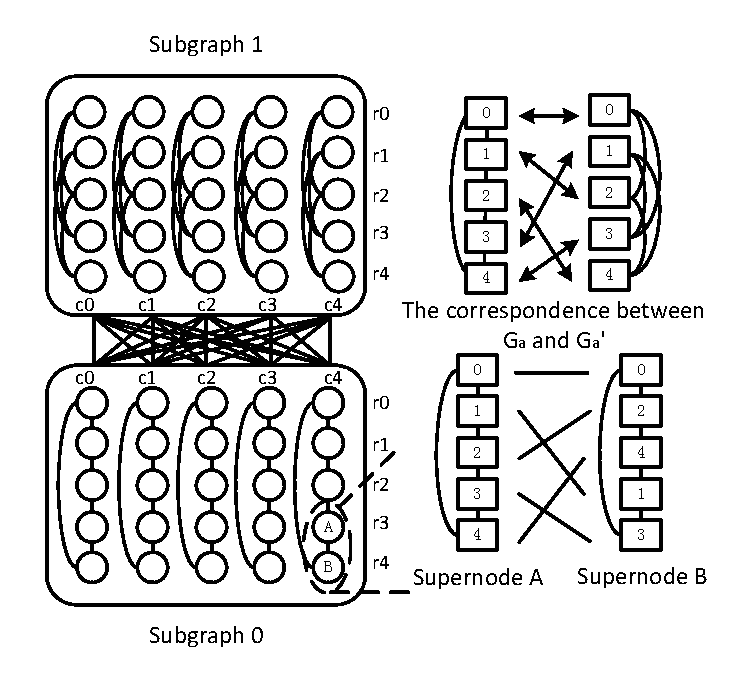
\includegraphics[width=.58\textwidth,height=.52\textwidth]{Visio-mpp_v1.eps}
  \vspace{-.3cm}
  \caption{Bundlefly}
  \label{mppv0}
\end{figure}

超级节点内部的链路取决于构造产生集合$X_{a}$,$X_{a}={1,\xi_{a}^{2},...,\xi_{a}^{a-3}}$ \upcite{GRMMS}。$\xi_{a}$是高斯域$\mathds{F}_{a}$的一个生成元。在$a$较小的时候,我们可以通过穷举搜索的方法找到一个生成元。 因此,超级节点内部的链路要遵循以下连接关系(所标注的算法都是需要进行模$a$的操作):

当且仅当$d_{4}-d_{4}'\in X_{a}$时,路由器$(d_{1},d_{2},d_{3},d_{4})$和路由器$(d_{1},d_{2},d_{3},d_{4}')$相连接。

在图\ref{mppv0}中,超级节点内有5个路由器。因此,高斯域$\mathds{F}_{5}$生成元为$\xi_{a}=2$而且$X_{a}=\{1,4\}$。超级节点$A$的路由器$(d_{1},d_{2},d_{3},0)$ 和超级节点$A$的路由器$(d_{1},d_{2},d_{3},4)$相连,是因为满足$d_{4}-d_{4}'= 0-4\ (mod\ 5)=1 \in X_{a}$。

MMS图决定了任意两个超级节点的连接关系,而函数$\phi$则决定了两个超级节点如何相连。超级节点是否连接满足以下条件\upcite{GRMMS}(所标注的算法都是需要进行模$q$的操作):

当且仅当$d_{2}-d_{2}'\in X_{q}$,超级节点$(0,d_{2},d_{3})$和超级节点$(0,d_{2}',d_{3})$相连;

当且仅当$d_{2}-d_{2}'\in X_{q}'$,超级节点$(1,d_{2},d_{3})$和超级节点$(1,d_{2}',d_{3})$相连;

当且仅当 $d_{2}=d_{3}*d_{3}'+d_{2}'$,超级节点$(0,d_{2},d_{3})$和超级节点$(0,d_{2}',d_{3}')$相连;

我们利用高斯域$\mathds{F}_{q}$的生成元$\xi_{q}$去构造两个生成集合$X_{q}$ 和$X_{q}'$ \upcite{GRMMS}。对较小的$q$值采用穷举算法找$\xi_{q}$是可行的。当$\delta=1$时,我们构造 $X_{q}=\{1,\xi_{q}^{2},...,\xi_{q}^{q-3}\}$和$X_{q}'=\{1,\xi_{q}^{3},...,\xi_{q}^{q-2}\}$。例如,当$q=5$时,$\xi_{5}=2$,则$X_{q}=\{1,4\}$和$X_{q}'=\{2,3\}$。在图\ref{mppv0}中,子图0每一列的超级节点之间连线取决于$X_{q}$。类似的,子图1的每一列的超级节点之间连线取决于$X_{q}'$。在\upcite{GRMMS}中,还介绍了在$\delta=0,-1$取值下$X_{q}$ 和$X_{q}'$的构造。

在Bundlefly的构造中,最难的是找到一个multi-star product方法对应的函数$\phi$以保证网络直径为3。如果两个超级节点在全局MMS 图中是相连的,那么,两个超级节点之间有$a$ 条链路,如图\ref{mppv0}中两个超级节点之间的连线所示。在介绍这$a$ 条链路如何相连之前,我们先介绍每个路由器的两套编号。一套是根据集合$X_{a}$。 另一套是根据集合$X_{a}'$通过使用函数$\phi$。 $G_{a}$和$G_{a}'$ 分别是集合$X_{a}$ 和$X_{a}'$的生成图。那么,$G_{a}$和$G_{a}'$互为同构图\upcite{GRMMS}。函数$\phi$是一个从$G_{a}'$ 映射到$G_{a}$的映射函数。如果$(u,v)$是$G_{a}'$的一条边,那么$(\phi(u),\phi(v))$则是$G_{a}$的一条边。如图\ref{mppv0}中$G_{a}$和$G_{a}'$的对应关系所示,$(0,2)$是$G_{5}'$的一条边,那么,其对应$G_{5}$ 的$(0,4)$。如果超级节点内的路由器编号为$\{0,1,2,3,4\}$,那么, $\phi(0,1,2,3,4)=\{0,2,4,1,3\}$则是路由器的另一套编号,如图\ref{mppv0}中
的函数$\phi$示意图所示。函数$\phi$不是唯一的,但是,我们只需要找到其中一个匹配即可。

为了超级节点间的具体连线,每一个超级节点都有一个编号($d_{1}*q^2+d_{2}*q+d_{3}$)。超级节点A$(d_{1},d_{2},d_{3})$和超级节点B$(d_{1}',d_{2}',d_{3}')$相连。如果超级节点A的编号大于超级节点B的编号,那么当且仅当 $d_{4}'=\phi(d_{4})$,超级节点A的路由器$(d_{1},d_{2},d_{3},d_{4})$和超级节点B的路由器$(d_{1}',d_{2}',d_{3}',d_{4}')$相连。如果超级节点A的编号小于超级节点B的编号,那么当且仅当 $d_{4}=\phi(d_{4}')$,超级节点A的路由器$(d_{1},d_{2},d_{3},d_{4})$ 和超级节点B的路由器$(d_{1}',d_{2}',d_{3}',d_{4}')$相连。在图\ref{mppvo}中,  函数$\phi(0,1,2,3,4)={0,2,4,1,3}$。超级节点A (0,3,4)小于超级节点B (0,4,4),那么, 由于$d_{4}=\phi(d_{4}')=\phi(3)=1$,路由器(0,3,4,1)与超级节点(0,4,4,3) 相连。

\section{Bundlefly的分析}
在本节我们根据常用的指标对Bundlefly(BF)进行分析,如:网络直径,可扩展性,二分带宽,最短路径的数量,平均距离和容错性。
我们比较BF和其他经典拓扑结构,如Dragonfly(DF)\upcite{dragonfly},Slim Fly (SF)\upcite{slimfly}等。

\subsection{网络直径}

Bundlefly的网络直径为3,是通过上面介绍的函数$\phi$获得的。使得网络直径为3 的最根本原因是因为任意两个相连的超级节点内的节点互相通信能够保证2跳内完成。任意两个相连的超级节点之间有$a$条链路。也就是,超级节点中每个路由器都有一条链路相连相邻超级节点的路由器。再加上,MMS图是一个直径为2的结构,那么,两个超级节点中的任意节点之间最多2 跳可达。每两个不相连的超级节点能够通过一个共同的相邻超级节点通信。如果两个路由器分别在两个不相连的超级节点内,第一步是先找到两个超级节点的公共超级节点。第二步是在公共的相邻超级节点内找到两个路由器中其中一个的相连节点。第三步是通过函数$\phi$找到相邻超级节点之间的路径。

函数$\phi$是根据Paley图同构的性质产生。超级节点内都是Paley图。根据Paley图的同构性,通过函数$\phi$从生成集$X_{a'}$映射到生成集$X_{a}$而改变路由器在超级节点内的编号。两个相连的超级节点A 和B,如图\ref{mppv0}所示,超级节点A 的编号$(d_{1},d_{2},d_{3})$小于超级节点B的编号$(d_{1}',d_{2}',d_{3}')$。 那么,超级节点A内的路由器使用生成集$X_{a}$产生的编号,而超级节点B内的路由器使用函数$\phi$生成的编号。超级节点B的编号小于超级节点A的编号的情况类似。超级节点A的路由器$(d_{1},d_{2},d_{3},d_{4})$ 和超级节点B的路由器$(d_{1}',d_{2}',d_{3}',d_{4}')$,如果$d_{4}-\phi(d_{4}')=0$,那么两个路由器直接相连。如果$d_{4}-\phi(d_{4}')\in X_{a}$,那么这两个路由器不直接相连,而且这个公共相邻路由器$(d_{1},d_{2},d_{3},\phi(d_{4}'))$在超级节点A 中。如果$d_{4}-\phi(d_{4}') \notin X_{a}$,那么,$d_{4}-\phi(d_{4}')\in X_{a}'$因为$X_{a} \cup X_{a}'=\mathds{F}_q-\{0\}$。这两个路由器不直接相连,而且这个公共相邻路由器$(d_{1}',d_{2}',d_{3}',x)$($d_{4}=\phi(x)$)在超级节点B中。因此,任意两个路由器分别在相连的两个超级节点内能够2跳内可达。所以,在Bundlefly结构中,任意两个
路由器3跳内可达。

\subsection{可扩展性}

随着当前网络规模增加的趋势,可扩展性对有效拓扑结构来说是一个重要的衡量指标。如果我们考虑更多的不同的应用模型,我们不仅要考虑网络的规模而且要考虑网络中机柜间的链路数量。在图\ref{constructdfv61}中,我们展示了不同拓扑结构在机柜间至少有4条链路条件下的可扩展性。这五个拓扑结构在使用端口数为48的路由器时,都不能构造出100K规模的系统。在Cray Cascasde系统\upcite{cascade} 中,每个路由芯片提供十条光链路,最多能连接960个超级节点。但是,为了增加超级节点间的链路带宽,就组合了每4条光链路捆在一起连接超级节点。那么,系统最多容纳241个超级节点。实际上,机柜间的带宽需求远远大于4条链路的带宽。由于多芯光纤的发展,多芯光纤的成本可以低于同等数量的单芯光纤的成本。在图\ref{constructdfv8}中,直径为3的SF和BF能够在使用48端口路由器的条件下构造100K规模的网络,而且能够提供10条以上的机柜间链路。在图\ref{constructdfv9} 中,展示了BF在参数$a$和$q$的不同配比下的可扩展性。在参数配比关系为$a=q$的条件下,可扩展性跟参数配比为$q-1=(a-1)/2$的可扩展性相近,而参数配比为$q-1=2a$条件下的可扩展性是三种配比关系中最低的。

\subsection{二分带宽}

如果网络采用随机分布的通信模式,二分带宽是理论上网络的最优吞吐率的上限。我们使用METIS划分工具\ref{METIS}去计算二分带宽。图\ref{bb}比较了不同拓扑结构的二分带宽。图\ref{bb0}展示的是在机柜间至少有一条单芯光纤的条件下,不同拓扑结构在不同的网络规模下二分带宽的趋势。BF和SF都属于机柜间有多条链路的结构。因此,图\ref{bb1}所示,使用多芯光纤(4芯光纤即机柜间至少有4条单芯光链路)的条件下,BF和SF跟在使用单芯光纤的条件下的二分带宽趋势一样。默认,BF的参数$a$和参数$q$的取值一样。 当BF的终端数$p$是路由器端口数的四分之一,那么BF获得最高的二分带宽,近似网络规模的五分之二。SF的二分带宽排第二,约网络规模的三分之一,比DF和Dragonfly+\upcite{Dragonfly+}以及终端数$p$ 是端口数的三分之一的BF的二分带宽高。在使用单芯光纤的DF+只能获得网络规模四分之一的二分带宽。DF+在使用多芯光纤条件下获得更高的二分带宽,约网络规模的七分之二。虽然在使用多芯光纤后增加了二分带宽,但是在使用同样端口数的路由器时,使用多芯光纤(每条多芯光纤含有l芯。)的DF+的规模将要减少到使用单芯光纤的规模的$1/l$。 使用多芯光纤的DF的二分带宽趋势和使用单芯光纤的DF的二分带宽的趋势基本一致。

\begin{figure}[t]
\setlength{\belowcaptionskip}{-.3cm}%
\centering
  \subfloat[Comparison of bisection bandwidth with SCF]{
    \includegraphics[width=.48\textwidth,height=.38\textwidth]{bbmetis1_0.eps}
  \label{bb0}
  }
  \subfloat[Comparison of bisection bandwidth with MCF(l=4)]{
    \includegraphics[width=.48\textwidth,height=.38\textwidth]{bbmetis1_1.eps}
    \label{bb1}
  }
  \vspace{-.3cm}
  \caption{二分带宽的比较}
  \label{bb}
\end{figure}

\begin{figure}[t]
\setlength{\belowcaptionskip}{-.3cm}%
  \centering
  \includegraphics[width=.48\textwidth,height=.3819\textwidth]{averagedistance.eps}
  \vspace{-.3cm}
  \caption{平均最短路径长度}
  \label{ad}
\end{figure}


\subsection{最短路径}

最短路径的数量是网络负载均衡的重要指标。要想获得较多的最短路径数量也是对路由器端口数、网络直径以及网络规模的一种权衡。
表\ref{Table2}展示了在同样的路由器规模下,不同拓扑结构的最短路径数量占比和路由器端口数。
$SP$是指最短路径数大于1的节点对占所有节点对($N_r\times(N_r-1)$)的比例。
尽管SF可以在给定路由器端口数的条件下构造更大的直径为2的拓扑结构,但是最短路径数量却小于其他拓扑结构,如表\ref{Table2}所示。
使用多芯光纤的DF(相当于任意两个超级节点之间有4条单芯光纤)获得最大的$SP$ 值。
但是,在同等路由器规模下,路由器端口数相当于两倍使用单芯光纤的DF和BF。
当DF和BF使用相近端口数的路由器构造相近规模的网络,BF能获得更高的$SP$。
在路由器规模为500时,BF的$SP$值高于使用多芯光纤的DF。如果$BF$的参数$a$取值大于5,
同一个超级节点内两个不相邻的节点之间至少2条最短路径。


\begin{table}[t]
\caption{最短路径数量}
\centering
\begin{tabular}{c| c| c |c|c|c|c|c}\hline
  \centering
  Topology & $k'$ & $N_r$ & SP & Topology & $k'$ & $N_r$ & SP \\
  \hline
  \multirow{3}*{SF}
  &25		&578	 &0.0139
  & \multirow{3}*{DF}
  &14		&550	&0.1744  \\
  &35 &1058  &0.0530 &
  &17	 &876	&0.1535 \\
  &47	&1922	 &0.0396  &
  &23		&2064	&0.1229   \\
  \hline
  \multirow{3}*{DF(MCF)}
  &23	 	&528	&0.6034
  & \multirow{3}*{BF}
   &15	 &686	&0.6904  \\

  &29	    &1020	&0.6634 &
  &19		&1210	&0.5644 \\
  &41	 &2772	&0.7449 &
  &23		&2662	&0.6521  \\
  \hline
\end{tabular}
\label{Table2}
\end{table}

\subsection{平均路径}

在BF中,任意两个终端的最短路径长度小于等于3跳。图\ref{ad}展示了不同拓扑结构在不同规模下的平均最短路径长度。
BF的平均最短路径长度小于3而且略小于使用单芯光纤DF的平均最短路径长度。使用多芯光纤的DF相比使用单芯光纤的DF
的平均最短路径长度要小,是因为使用了更多端口数连接其他路由器。

\subsection{容错性}

我们使用链路的出错概率,平均路径长度以及网络直径来分析拓扑结构的容错性。
在链路随机出错情况下,我们模拟分析了平均路径长度和网络直径是如何变化的。我们采用删除结构中链路使得网络不连通的方式衡量网络的容错性。表\ref{Table3}中展示了不同拓扑结构在路由器规模为500和1000的情况下的容错性。随着网络规模的增加,容错性也随之增强。
SF 是所比较的拓扑结构中容错性最好的结构。主要原因是因为SF具有更短的网络直径以及每个节点的端口数多。
在路由器规模为500的条件下,使用多芯光纤的DF中每个路由器有23个相邻路由器。
在路由器规模500的条件下,SF中的每个路由器有25个相邻路由器。但是,BF则只有13个路由器,只有SF和多芯光纤的DF路由器端口数的$50\%$。
在路由器规模为1000的条件下,在SF 和使用多芯光纤的DF中的路由器分别有35个和29个相邻的路由器。
然而,在BF和使用单芯光纤的DF 中,每个路由器分别只有19和20个相邻路由器。
在图\ref{r}中我们展示了在链路不同程度的出错情况下,BF的网络直径和平均路径长度的变化。在路由器规模为1000的条件下,随着出错概率的增加,平均路径长度从2.72增加到4.15而网络直径从3增加到8。


\begin{figure}[t]
\setlength{\belowcaptionskip}{-.3cm}%
  \centering
 \begin{minipage}[t]{\textwidth}
   \centering
  \subfloat[Average path length]{
    \includegraphics[width=.46\textwidth,height=.38\textwidth]{resiliency0.eps}
  \label{r0}
  }
  \subfloat[Diameter]{
    \includegraphics[width=.46\textwidth,height=.38\textwidth]{resiliency1.eps}
    \label{r1}
  }
  \vspace{-.3cm}
  \caption{不同链路错误率}
  \label{r}
  \end{minipage}

\end{figure}

\begin{table}[t]
\caption{不同拓扑结构的容错性}
\centering
\begin{tabular}{c|c| c| c |c }\hline
  \centering
  $N_r$ & SF &DF &DF(MCF) &BF	\\\hline
  $0.5K$ &65\%  &55\%  &65\% &60\%\\
  $1K$	&80\%	&65\%  &75\% &65\% \\\hline
\end{tabular}
 \label{Table3}
\end{table}

\section{路由算法}
\label{routingalgorithm}

我们将在本节介绍Bundlefly的最短路径和非最短路径以及我们设计的自适应路由算法。我们还介绍了Bundlefly是如何进行死锁避免的。

\subsection{最短路径路由}

Bundlefly的最短路径路由(MIN)是一个层次化路由。首先,我们要先确定当前超级节点和目的超级节点在MMS图中的位置。
第二,我们需要确认当前路由器和目的路由器在超级节点内的位置。最后,我们要找到从当前路由器的出去的端口。

一个报文从源终端所在的超级节点$S_s$的源路由器$R_s$注入并被目的终端所在的超级节点$S_d$的目的路由器$R_d$所吸收。
图\ref{ra}中展示了最短路径路由算法最典型的三种情况。
当$S_s=S_d$时,我们可以不用确定当前超级节点的位置直接确定当前路由器和目的路由器在超级节点内的位置,如图\ref{ra2}所示。
Paley graph是一个直径为2的拓扑结构。因此,报文从路由器$R_s$路由到路由器$R_d$在两跳之内。如果$S_s \neq S_d$,我们分析两个超级节点是否在MMS图中相连。如果$S_s$和$S_d$不相连,我们需要找到一个公共相邻超级节点$S_i$作为中转的一步,如图\ref{ra0}所示。MMS图是一个直径为2的拓扑结构,因此我们肯定可以找到一个公共的相邻超级节点。根据超级节点在MMS图中的不同位置,可能存在多于一个的公共相邻超级节点。由于,路由器在超级节点内的位置不同,选择不同的公共相邻超级节点,路径长度可能会不一样,2跳或者3跳。在路径长度为3的情况下,两个不相连的超级节点之间通信如图\ref{ra0}所示。先将报文发送给公共相邻超级节点$S_i$ 中$R_s$ 的相邻节点$R_a$。每个路由器都有一条链路连接相邻超级节点内的路由器。当报文到达公共相邻超级节点$S_i$后,路由算法与$S_s$和$S_d$相连的情况相同。当$S_s$跟$S_d$ 相连,$R_s$和$R_d$相距要么1跳或者2跳,如图\ref{ra1}所示。正如前面讨论的如果两个超级节点相连,两个超级节点内的路由器互相通信可以根据函数$\phi$找到路径。

当参数$a$即超级节点内的路由器数量大于5时,而且$R_s$和$R_d$在同一个超级节点不相连,那么$R_s$和$R_d$之间至少有2个公共相邻路由器。如果参数$q>5$且满足$\delta=1$,而且$S_s$和$S_d$在MMS图中的同一个组内,那么,$S_s$和$S_d$ 之间至少有2个公共相邻超级节点。



\begin{figure}[t]
\setlength{\belowcaptionskip}{-.5cm}%
\centering
  \subfloat[$S_s$与$S_d$不相连]{
    \includegraphics[width=.44\textwidth,height=.40\textwidth]{Visio-routing_0.eps}
  \label{ra0}
  }
  \subfloat[$S_s$与$S_d$相连]{
    \includegraphics[width=.30\textwidth,height=.40\textwidth]{Visio-routing_1.eps}
  \label{ra1}
  }
  \subfloat[$S_s=S_d$]{
    \includegraphics[width=.2\textwidth,height=.36\textwidth]{Visio-routing_2.eps}
    \label{ra2}
  }
  \vspace{-.3cm}
  \caption{Bundlefly的路由算法}
  \label{ra}
\end{figure}

\subsection{非最短路径自适应路由}

我们在本节介绍Bundlefly的非最短路径路由算法(NONMIN)。非最短路径路由可以用来均衡高负载最差通信负载,而最短路径路由则不能很好的做到。在NONMIN路由算法中,报文在源路由器$R_s$随即选择一个路由器$R_i$(既不是$R_s$也不是$R_d$)作为中间目的节点。首先,报文从$R_s$到$R_i$走最短路径路由。第二步,
报文从$R_i$到$R_d$走最短路径路由。NONMIN路由算法的路径由两段最短路径路由组成。因此,一条NONMIN路由的路径长度一般2-6跳。不同的跳步数取决于$R_s$,
$R_i$以及$R_d$之间的距离。

我们设计的非最短路径自适应路由(NMA)就是基于缓存区队列长度选择走最短路径路由或是非最短路径路由。$Q_{min}$是最短路径路由端口的缓冲区队列长度。$Q_{nonmin}$则是非最短路径路由端口的缓冲区队列长度。我们还相应的设置了队列的阀值来决定走哪一条路径,$T_{min}$和$T_{nonmin}$。如果$Q_{nonmin}<Th_{nonmin}$而且$Q_{min}>Th_{min}$,那么报文选择NONMIN路由。
其中,$T_{min}$和$T_{nonmin}$的取值根据多次模拟获得。我们设置$Th_{nonmin}=1.5\times Q_{min}$以及$Th_{min}=0$。在Bundlefly结构中,NONMIN的路径长度不仅可能会导致加剧网络拥塞,而且,需要更多的虚拟通道来避免死锁。 因此,在大多数情况下,一般限制路径的长度在可允许的虚拟通道
(Virtual Channel(VC))的数量范
围内。例如,我们限制路径长度不超过4跳,那么,报文从$R_s$到$R_i$这一段的路由只走1跳,接下来,报文直接从当前路由器执行最短路径路由到$R_d$。

\subsection{死锁避免}

Bundlefly的死锁避免机制采用的是每一跳切换一条VC使得链路之间不形成依赖环。Bundlefly是一个直径为3的拓扑结构,因此,MIN最多只需要3条VC就可以避免死锁,而NONMIN在不限制路径长度的情况下需要6条VC,NMA则需要4条VC(因为路径长度限制在4跳内)。但是,Bundlefly是一个直径为3的层次化结构,我们可以像Dragonfly\upcite{dragonfly}结构一样利用层次化降低对VC的需求。

在MIN中,一个报文最多经过两条超级节点之间的链路和一条超级节点内部的链路,或者一条超级节点之间的链路和一条超级节点内部的链路,或者两条超级节点内部的链路,或者一条超级节点内部的链路,或者一条超级节点之间的链路。
图\ref{ra}展示了路由路径的三种典型情况。在Bundlefly结构中,不存在经过3条超级节点之间的链路也不存在经过三条超级节点内部的链路。而且,所有MIN路径
若有的话都是先使用超级节点之间的链路然后在使用超级节点内的链路。
所以,一条VC可以被同时使用于超级节点之间的链路和超级节点内部的链路,如图\ref{ra}所示。当$S_s$和$S_d$不相连,如图\ref{ra0}所示,从$R_s$到$R_d$
的报文路由到公共相邻超级节点$S_i$的$R_a$,所经过超级节点之间的链路采用的是$VC_0$。那么,从$S_i$到$S_d$报文所经过超级节点之间的链路则采用的是$VC_1$。最后,报文在$S_d$内到达$R_d$所经过的超级节点内部的链路采用的是$VC_0$。VC的数量从3条减少到2条。对于NONMIN来说,我们至少需要4条VC来避免死
锁。对NMA来说,如果限制路径长度在4跳以内,那么,使用3条VC能够避免死锁。因为NMA最多经过3条超级节点内链路或者超级节点之间链路。

\section{性能分析}
在这一章节中,我们使用一个时钟精确的网络模拟器Booksim\upcite{Booksim}模拟Bundlefly (BF)和其他拓扑结构并且通过一个伯努力分布报文注入模型分析不同
拓扑结构的性能。首先,我们在几种典型的通信模式下评测了BF并与其他拓扑结构
进行了比较。第二,我们比较了BF的不同配置的路由算法在不同的通信模式下的
性能。第三,我们提出了一个物理布局并评测了不同拓扑结构在这种物理布局下性的性能。最后我们分析了BF在物理布局条件下不同参数配置的性能。

\textbf{路由器:}我们使用了传统的具备完整的路由器流水线的输入队列(input-queue (IQ))路由器模型。路由器是基于Virtual Cut-through(VCT)交换机
制。我们假设信用处理过程需要2个时钟周期,路由计算模块需要2个时钟周期,以及交换分配模块,虚通道(VC)分配模块和crossbar处理模块都需要1个时钟周期。crossbar的输入和输出的加速比都是1。内部传输数据链路数率是链路传输速率的两倍。

\textbf{网络:} 我们提供了两种链路传输延迟的配置。一种是每一条链路的传输延迟都是1个时钟周期。根据这种配置,我们可以减少不同拓扑结构在构造同等规模的网络时使用不同端口数的路由器而造成的影响并观察网络状态。在\upcite{slimfly}
和\upcite{dragonfly}中,链路传输延迟也是设置为1个时钟周期。另外一种配置是为
了模拟实际系统物理布局而根据物理布局中的位置设置延迟。机柜间链路包括路由
器流水线的延迟一共100个周期,而机柜内链路则是50个周期。报文长度默认是1个
切片大小。每个端口的缓冲区容量是256个切片。缓冲区的管理机制采用每个VC拥有
5个切片的私有存储空间,其他的缓冲区由所有VC共享。网络的规模约为$N\approx10K$以及不同的拓扑结构在规模上的差别控制在10\%以内。我们将BF和Flattened Butterfly(FB),Dragonfly(DF)和Slim Fly(SF)进行比较。拓扑结构的具体配置如表\ref{Table6}所示。供给比例(oversupply)是指最小二分的链路切割数和网络规模的一半的比值。FB和DF都是典型的直径为3的高阶直接互连网
络。SF是最新的性价比高的低延迟直接互连网络。如果我们使用端口数为25的路由器构建网络,使用FB和SF结构不能搭建出10K规模的网络。在设置配置上我们是在路由器个数和路由器端口数以及供给比例之间作权衡。因此,我们给BF设置了两种配置。

\textbf{路由算法:}我们比较了不同拓扑结构在使用以下路由算法的性能:DF\upcite{dragonfly},FB\upcite{Flattenedbutterfly}以及SF\upcite{slimfly}的最短路径路由(MIN)和基于本地缓冲区队列大小的全局自适应负载均衡路由算法(UGAL)。对于BF,我们分析了MIN、NONMIN以及NMA在不同的通信模式下的性能。

\textbf{通信模式:}我们考虑了采用典型的通信模式去评测不同的拓扑结构,
如均衡随机通信模式和最差通信模式。针对物理布局,我们还设计了全局最差通信模式去研究和分析拓扑性能。

\begin{table}[t]
 \centering
%\setlength{\belowcaptionskip}{-.5cm}%
%\captionof{table}{The configurations of Bundlefly, Flattened Butterfly, Slim Fly, and Dragonfly. (Cabs abbreviated for cabinates)}
\caption{Bundlefly、Flattened Butterfly、Slim Fly和Dragonfly的配置}
\centering
\begin{tabular}{c| c| c|c|c| c }\hline
  \centering
  拓扑	& $k$ &$p$ & $N_r$ &\tabincell{c}{Over-\\supply} & 机柜  \\\hline
  FB &37 &10	   &1000	&0.51 &10 	 \\\hline
  DF &27 &7	&1386	&0.50 &11	  \\\hline
  SF &43 &14 	&722	&0.68 &19  	 \\\hline
  BF0 &25 &8 	&1274 	&0.48 &7	\\\hline
  BF1 &25 &6 	&1666 	&0.63 &7   \\\hline
\end{tabular}
\label{Table6}
 \end{table}


\subsection{物理布局}

如何在布局一个低直径网络的同时使用最少的缆线开销是高性能计算系统和数据中
心系统实际物理部署时具有挑战的工作\upcite{slimfly}。设计Bundlefly的初衷就是
构造一个多芯光纤友好的拓扑结构,为了可维护性和高效的成本开销利用多芯光纤代替传统的一捆单芯光纤。我们给Bundlefly设计了一个布局模型,充分关注多光纤的好处。

在\upcite{slimfly}中,Slimfly根据MMS图的模块结构被划分。在Bundlefly中,同样
可以根据MMS图的模块结构划分并充分使用多芯光纤。如果$d_1\neq d_1'$并且$d_3=d_3'$ ,那么MMS图中不同子图的两个组被封装在同一个机柜内。机柜的布局
是一个全互连网络而且任意两个机柜之间有$2\times q \times a$条链路,
如图\ref{mpplayout}所示。对于Dragonfly结构,我们封装9个超级节点在同一个机
柜中。对于Flattened Butterfly结构,我们封装两维的路由器在同一个机柜中。
不同的拓扑结构具体布局配置如表\ref{Table6}所示。每个拓扑结构的机柜布局都是全互连网络以及每个机柜在网络中都是同样的构造单元。对不同的拓扑结构:Flattened Butterfly,Dragonfly,Slim Fly,Bundlefly0和Bundlefly1,任意两个机柜间的链路分别是100、81、38、182和238。

\begin{figure}[t]
\setlength{\belowcaptionskip}{-.5cm}%
  \centering
    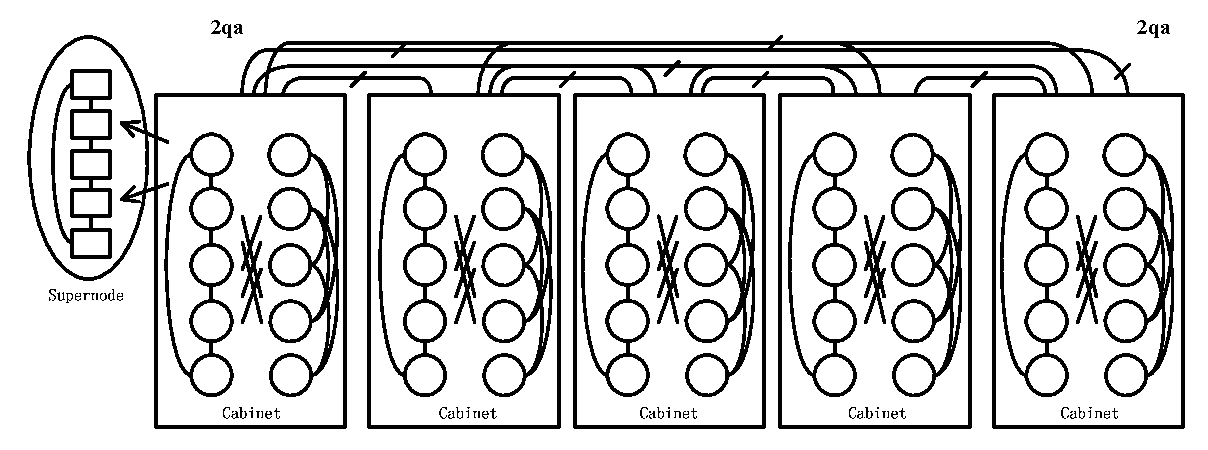
\includegraphics[width=.8\textwidth,height=.33\textwidth]{Visio-mpp_layout.eps}
  \vspace{-.3cm}
  \caption{Bundlefly的物理布局}
  \label{mpplayout}
\end{figure}

\subsection{均衡随机通信模式}

在均衡随机通信模式下,每个报文的源节点和目的节点都是随机生成。
图\ref{l1un}展示了不同拓扑结构在使用最短路径路由的性能。因为采用的是
链路传输延迟为1个时钟周期的配置,所以零负载情况下的延迟小于20个时钟周期。
正如预期所推测的一样,BF1的性能是五种拓扑结构中最好的,如图\ref{l1un_0}所示。BF1的供给比例比FB、DF以及BF0都要高。而且BF1的链路数是所有拓扑结构里最
多的。但是,BF1的路由器端口数却是所有拓扑结构中使用的最少的,BF0也是使用
同样端口数的路由器。相比较较少端口数的路由器,因为原本是路由器之间的链路变成路由器内部的链路,更高阶的路由器能够获得更好的性能。如图\ref{l1un}所
示,FB和SF使用更高阶的路由器获得比DF和BF0更好的性能。FB使用比BF0的路由器多$48\%$端口的路由器获得了比BF0高$27\%$的性能。SF则使用了比BF0的路由器多$72\%$端口的路由器获得了比BF0高$33.3\%$的性能。SF的延迟低于BF因为SF的直径
更低。尽管SF的供给比例更高,但是它跟BF1的饱和点一样。BF0比DF少使用了
$7\%$的路由器数量和$22\%$的链路却获得了高$7\%$的性能。

图\ref{layoutun}展示了物理布局配置的链路传输延迟的拓扑结构在均衡随机通信模式下的性能。拓扑结构展示了跟链路传输延迟为1个时钟周期的网络相似的性能趋
势。BF的延迟略高于其他拓扑结构是因为在使用最短路径路由算法的情况下,两个不相邻的超级节点可能需要经过2条机柜间链路。


\begin{figure}[t]
%\setlength{\belowcaptionskip}{-.5cm}%
  \centering
 \begin{minipage}[t]{\textwidth}
   \centering
  \subfloat[DF, FB and BF]{
    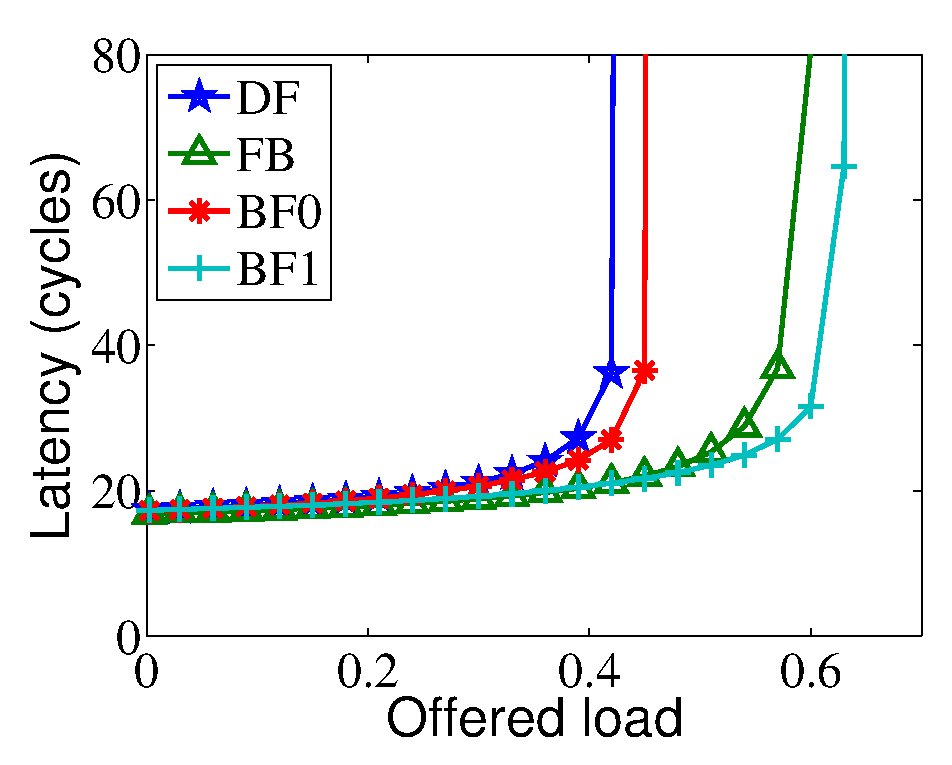
\includegraphics[width=.46\textwidth,height=.38\textwidth]{l1un0.eps}
  \label{l1un_0}
  }
  \subfloat[SF and BF]{
    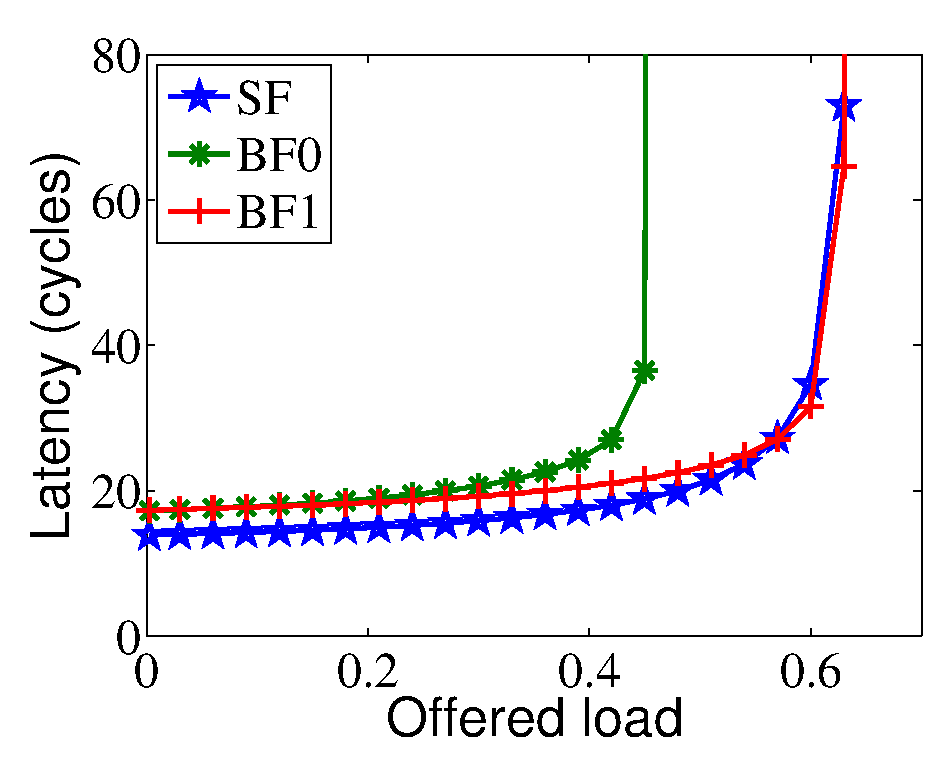
\includegraphics[width=.46\textwidth,height=.38\textwidth]{l1un1.eps}
    \label{l1un_1}
  }
  \vspace{-.3cm}
  \caption{均衡随机通信模式}
  \label{l1un}
  \end{minipage}
\end{figure}

\begin{figure}[t]
\setlength{\belowcaptionskip}{-.3cm}%
  \centering
 \begin{minipage}[t]{\textwidth}
   \centering
  \subfloat[DF, FB and BF]{
    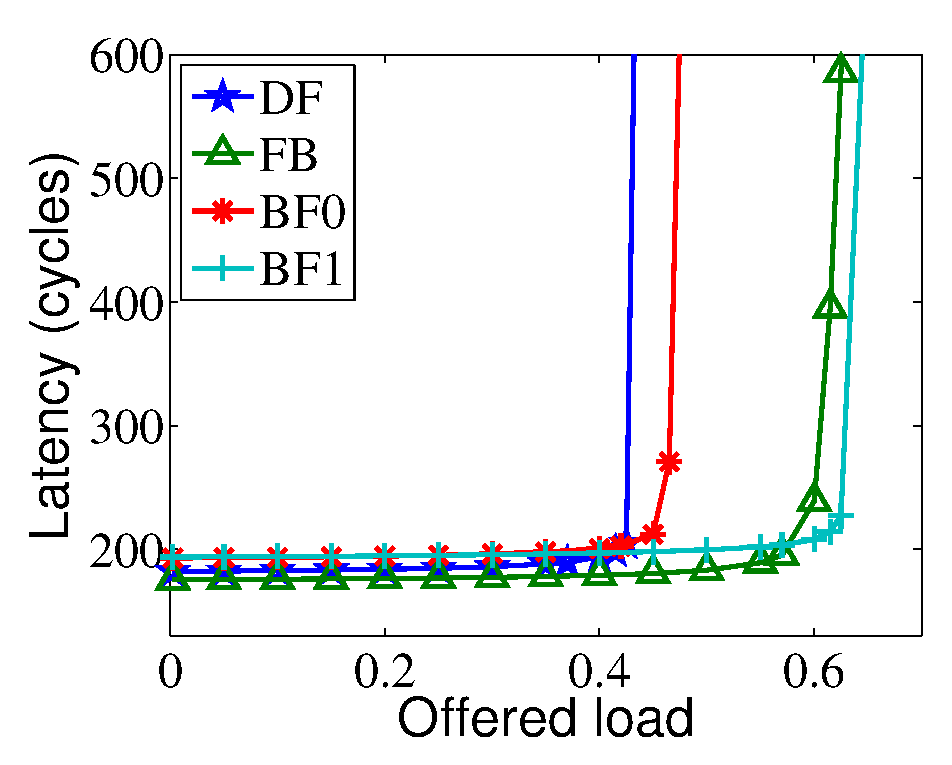
\includegraphics[width=.46\textwidth,height=.38\textwidth]{l1un10K0.eps}
  \label{layout_un0}
  }
  \subfloat[SF and BF]{
    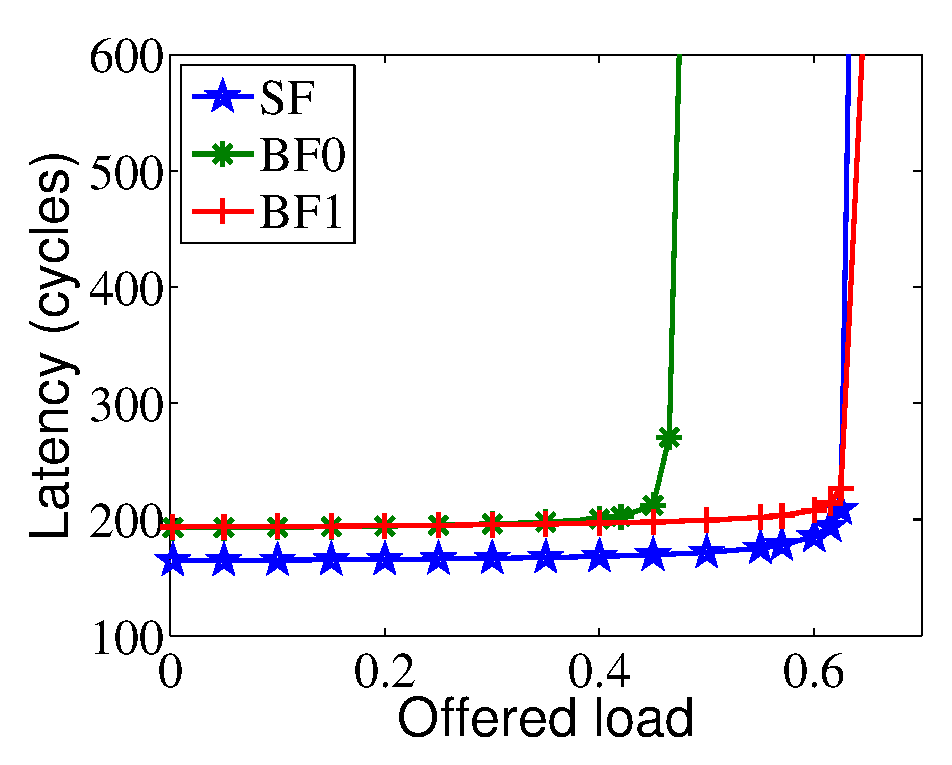
\includegraphics[width=.46\textwidth,height=.38\textwidth]{l1un10K1.eps}
    \label{layout_un1}
  }
  \vspace{-.3cm}
  \caption{物理布局下均衡随机通信模式}
  \label{layoutun}
  \end{minipage}
  \end{figure}

  \subsection{最差通信模式}

  我们给每一种拓扑结构都定义了一种最差通信模式,在这种模式下,报文的源节点和目的节点都相距最长距离。而且,部分链路会因为根据拓扑结构的特点设置
  的通信模式而发生拥塞。在DF结构中,报文的源节点和目的节点分别在两个确定
  的超级节点之间,这样会导致两个固定超级节点之间的链路和超级节点内部的链路拥塞\upcite{dragonfly}\upcite{OFAR}。 在SF结构中,报文通信只在MMS图同一个子图内2个确定的组之间产生\upcite{slimfly}。同一个子图内的两个组是不相连的。因此,通信需要一个在另一个子图的公共相邻路由器。对于FB结构,最差通信模式类似于$k-ary$ $n-cube$网络的飓风模式,报文产生于两个不同的维度并
  导致维与维之间的链路拥塞。对于BF结构,我们安排源节点和目的节点分别在两个确定的超级节点内,这两个超级节点在MMS图同一个子图不同组内。BF的最差通信模式类似于SF和DF,如图\ref{ra0}所示,$S_s$内的所有路由器向$S_d$内的所有路由器发送报文,而且这种情况下,$S_i$是$S_s$和$S_d$唯一的公共相邻超级节点。在最差通信模式下,DF、FB和SF 采用的是UGAL路由算法,而BF则采用的是
  NMA路由算法。

  图\ref{adv}展示了最差通信模式下不同拓扑结构的性能。链路传输延迟为1个时
  钟周期。DF的性能是五种拓扑结构中最差的,因为,任意两个超级节点之间只有一条链路。即使采用了UGAL路由算法,超级节点间的链路的高负载会造成整个网络迅速拥塞。FB结构的性能比BF0的性能低$30\%$。FB中每个路由器都有一条链路连接另一维的路由器。这种集中的通信造成维与维之间的链路拥塞。SF、BF0和BF1都展现了比DF和FB更好的性能。SF中的两个组之间是不相连的,路经长度至少是2。但是,每一对源节点和目的节点都有他们自己的公共相邻路由器,这有助于
  负载均衡。再加上,SF的网络直径最小,其饱和点最高而且延迟最低。但是在注
  入率为0.28时,SF的延迟突然变高,这主要是网络中负载增加网络路由策略变成
  非最短路径路由。在BF结构中,两个超级节点也是不相连,所以路径长度也是至少2跳。在最短路径路由时,每一对源节点和目的节点都是通过同一个公共相邻超级节点的路由器中转。但是这个公共相邻超级节点能够通过源超级节点和中转超级节点之间的多条链路减轻拥塞。

  \begin{figure}[t]
\setlength{\belowcaptionskip}{-.5cm}%
  \centering
 \begin{minipage}[t]{\textwidth}
   \centering
  \subfloat[DF, FB and BF]{
    \includegraphics[width=.46\textwidth,height=.38\textwidth]{advl110k0.eps}
  \label{adv0}
  }
  \subfloat[SF and BF]{
    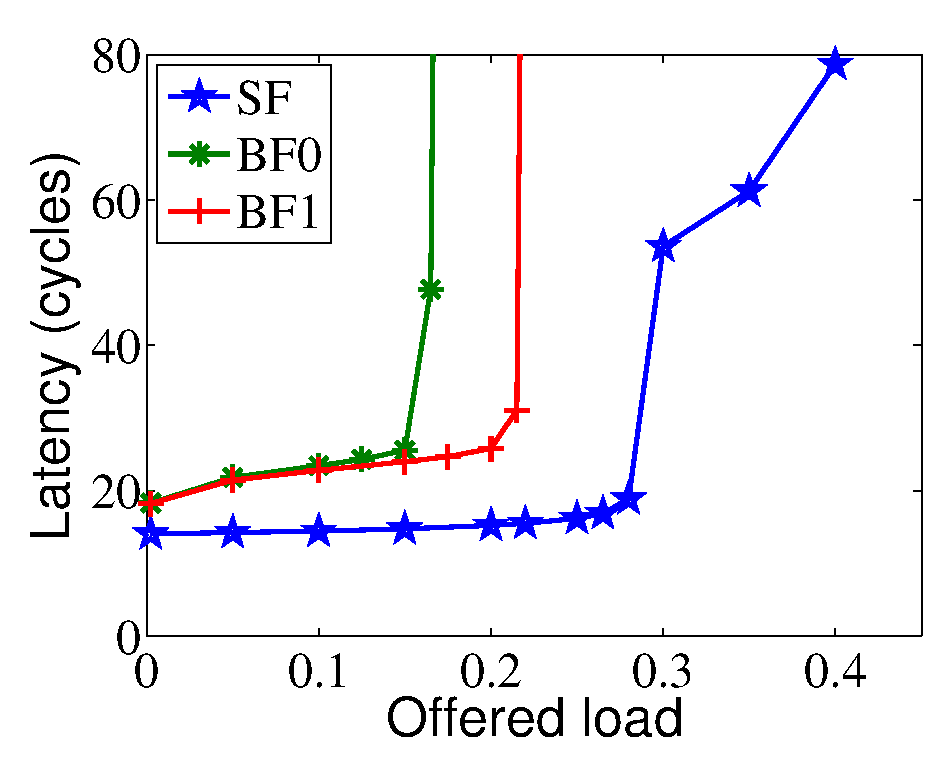
\includegraphics[width=.46\textwidth,height=.38\textwidth]{advl110k1.eps}
    \label{adv1}
  }
  \vspace{-.3cm}
\caption{最差通信模式}
  \label{adv}
   \end{minipage}
    \end{figure}

\subsection{全局最差通信模式}

在全局最差通信模式下,报文的源节点和目的节点分别来自两个确定连续的集合。
而且,集合的规模取决于每个拓扑结构机柜的大小如表\ref{Table6}所示的拓扑配
置。如果一个机柜的大小为$x$,那么按编号前x个终端给后x个终端发送报文。在DF 结构中,每9个超级节点882个终端被封装在同一个机柜中。在FB结构中,每个集合
有两维路由器共1000个终端组成。在BF结构中,每个集合有$2\times q$个超级节点即14 个
超级节点,那么BF0中的一个集合有1456个终端,BF1则有1428个终端。在SF结构
中,每个集合有532个终端。

首先,我们评测了链路传输延迟为1个时钟周期的实验结果,如图\ref{l1adv}所示。BF0和BF1的饱和点比FB以及DF都要高,有两个主要原因。一是两个集合间链路最多能达到$2\times q\times a$条链路。DF和FB的两个集合间链路较少使得饱和点
低。DF结构在最短路径路由策略下882个终端竞争81条链路。FB结构在最短路径路由策略下1000个终端竞争100条链路。SF和BF在图\ref{l1adv}中都展现了较好的性能。在SF和BF结构中,源节点和目的节点的公共相邻路由器一般都在其他集合。因此,另一个原因就是SF和BF可以不受限于两个集合之间的链路而且能较好的均衡负载。从注入率0.06到0.2,SF的延迟先升后降。这个主要原因是为了缓解网络拥塞切换了路由算法。在注入率0.06刚开始时,网络通过观察缓冲区注入率认为网络即将拥塞,路由策略从最短路径路由切换到非最短路径。实际上,这个拥塞只是短暂的
随后拥塞现象缓解,路由算法又切换回最短路径路由。

图\ref{layoutgla}展示的是根据物理布局配置链路传输延迟的网络的实验结果。机柜间延迟是机柜内延迟的两倍。BF的大多数报文都要路由经过两条机柜间链路和一条机柜内链路。尽管BF的延迟略高于其他拓扑结构,但是BF的饱和点却比别的拓扑结构好,特别是BF1。SF的饱和点比BF1的要低,因为BF1的机柜间链路比SF链路多。

\begin{figure}[t]
\setlength{\belowcaptionskip}{-.5cm}%
  \centering
 \begin{minipage}[t]{\textwidth}
   \centering
  \subfloat[DF, FB and BF]{
    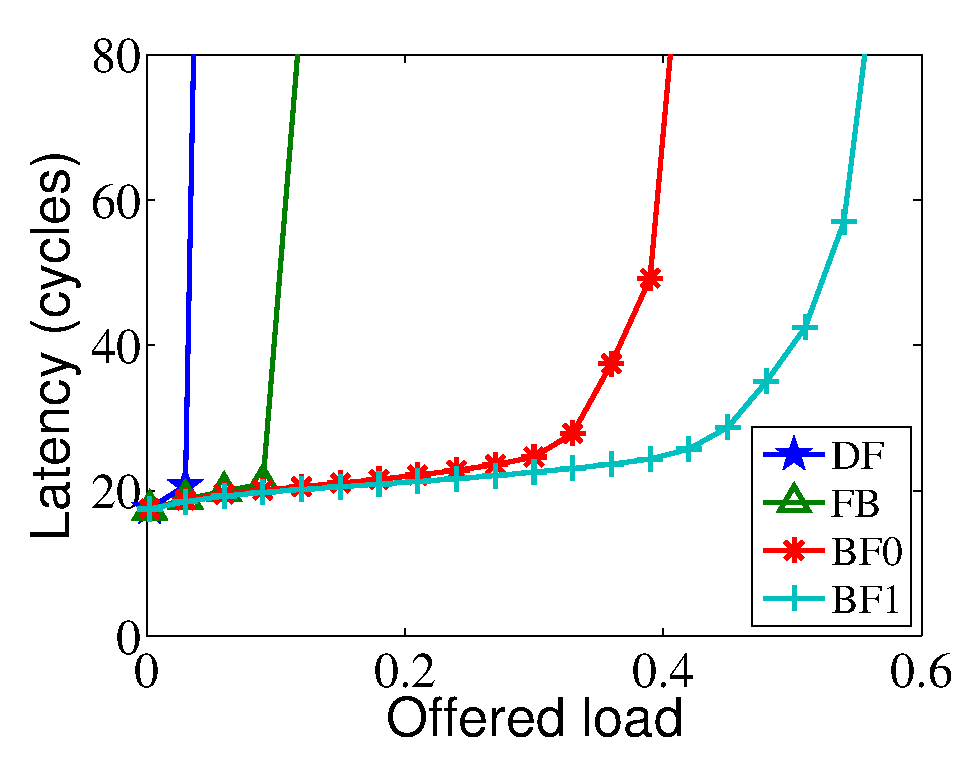
\includegraphics[width=.46\textwidth,height=.38\textwidth]{l1adv0.eps}
  \label{l1adv_0}
  }
  \subfloat[SF and BF]{
    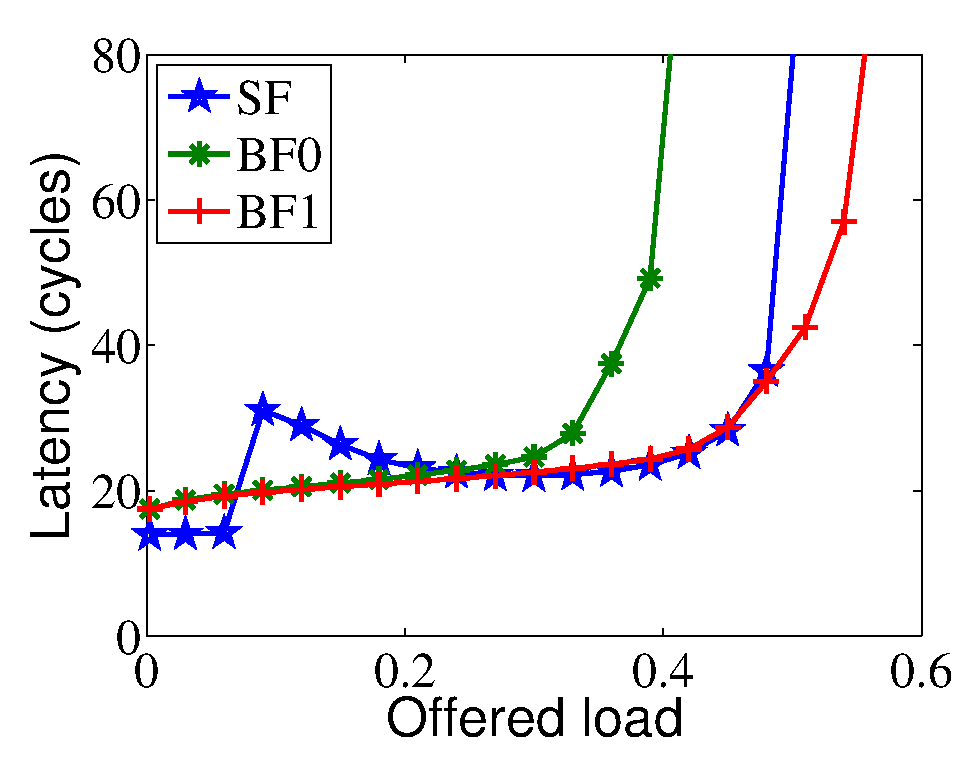
\includegraphics[width=.46\textwidth,height=.38\textwidth]{l1adv1.eps}
    \label{l1adv_1}
  }
  \vspace{-.3cm}
  \caption{全局最差通信模式}
  \label{l1adv}
  \end{minipage}
 \end{figure}

 \begin{figure}[t]
 \setlength{\belowcaptionskip}{-.5cm}%
  \centering
 \begin{minipage}[t]{\textwidth}
   \centering
  \subfloat[DF, FB and BF]{
    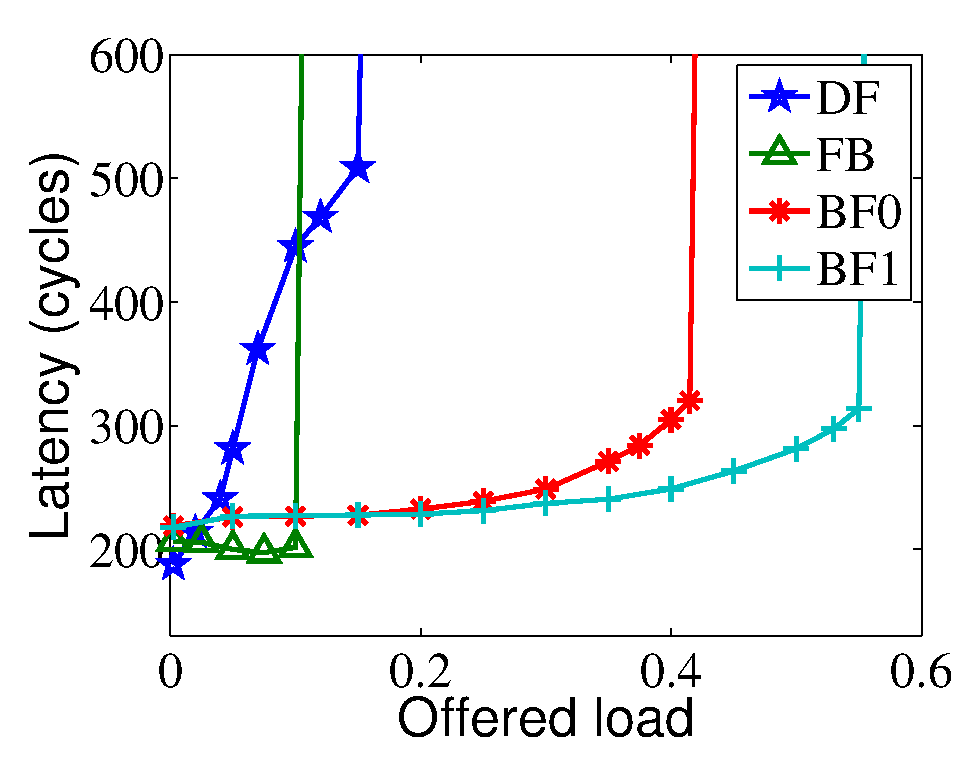
\includegraphics[width=.46\textwidth,height=.38\textwidth]{l1adv10K0.eps}
  \label{layout_gla0}
  }
  \subfloat[SF and BF]{
    \includegraphics[width=.46\textwidth,height=.38\textwidth]{l1adv10K1.eps}
    \label{layout_gla1}
  }
  \vspace{-.3cm}
  \caption{物理布局下最差通信模式}
  \label{layoutgla}
  \end{minipage}
  \end{figure}

  \subsection{不同的路由算法}

图\ref{l1ra01}和图\ref{l1ra02}展示了四种路由算法的性能。NONMIN被限制在4跳以内,NMA0也被限制在4跳以内,NMA1被限制在5跳以内。我们采用了物理布局链路传输延迟的配置去模拟不同的路由算法并分析其区别。在均衡负载模式下,无论BF 的什么拓扑配置,NONMIN都是延迟最高的路由算法,因为,NONMIN执行的是确定性绕路路径。因为路径长度最短,MIN是获得延迟最小的路由算法。NMA0和NMA1的区别
很小。在全局最差通信模式下,MIN的饱和点最小。在较低的注入率时,NMA0和NMA1
的延迟低于NONMIN但是高于MIN。NMA0的延迟比NMA1小是因为在较高负载下NMA0的绕路路径更短。

  \begin{figure}[t]
\setlength{\belowcaptionskip}{-.5cm}%
  \centering
 \begin{minipage}[t]{\textwidth}
   \centering
  \subfloat[BF0]{
    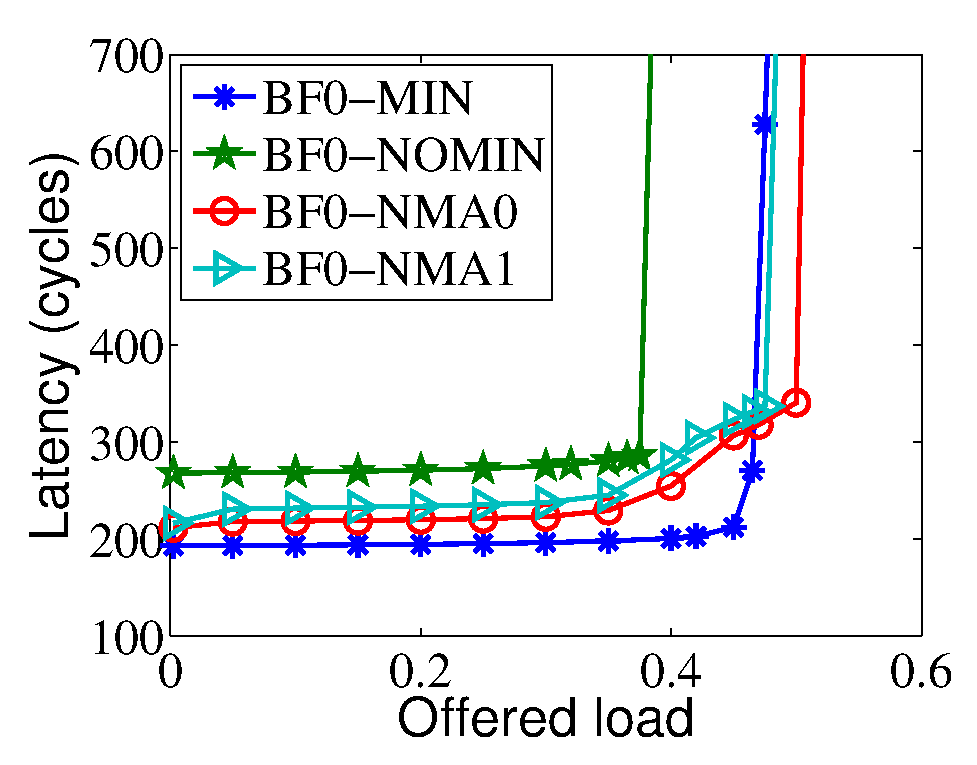
\includegraphics[width=.46\textwidth,height=.38\textwidth]{routing10Kun0.eps}
  \label{routing0}
  }
  \subfloat[BF1]{
    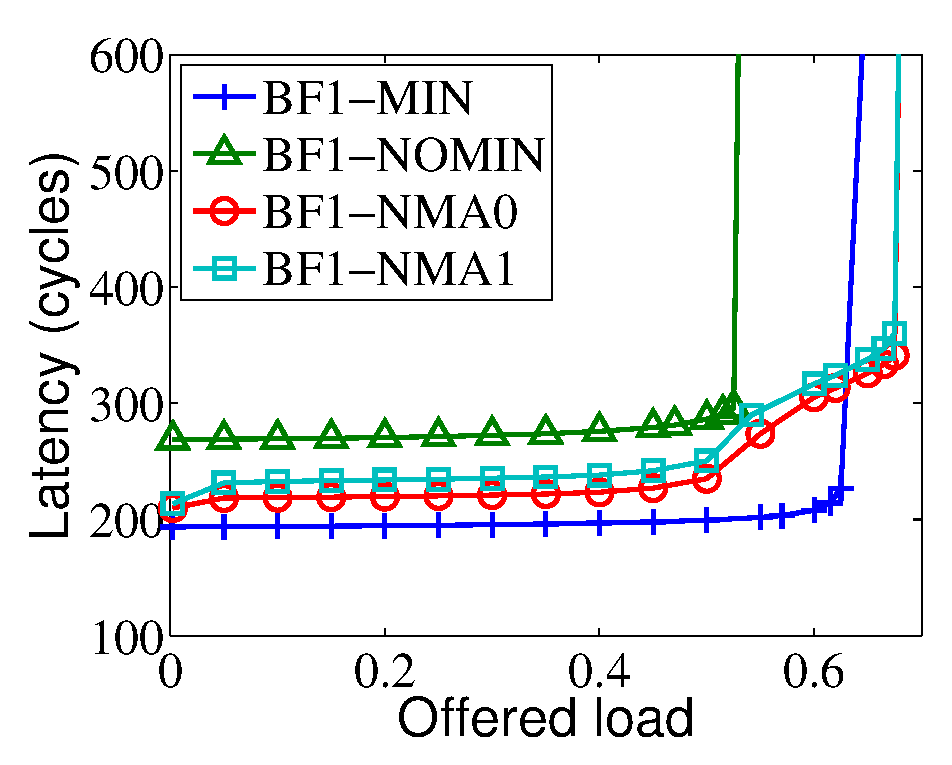
\includegraphics[width=.46\textwidth,height=.38\textwidth]{routing10Kun1.eps}
    \label{routing1}
  }
  \vspace{-.3cm}
  \caption{均衡通信模式下不同路由算法性能}
  \label{l1ra01}
  \end{minipage}
  \end{figure}

   \begin{figure}[t]
\setlength{\belowcaptionskip}{-.5cm}%
  \centering
 \begin{minipage}[t]{\textwidth}
   \centering
  \subfloat[BF0]{
    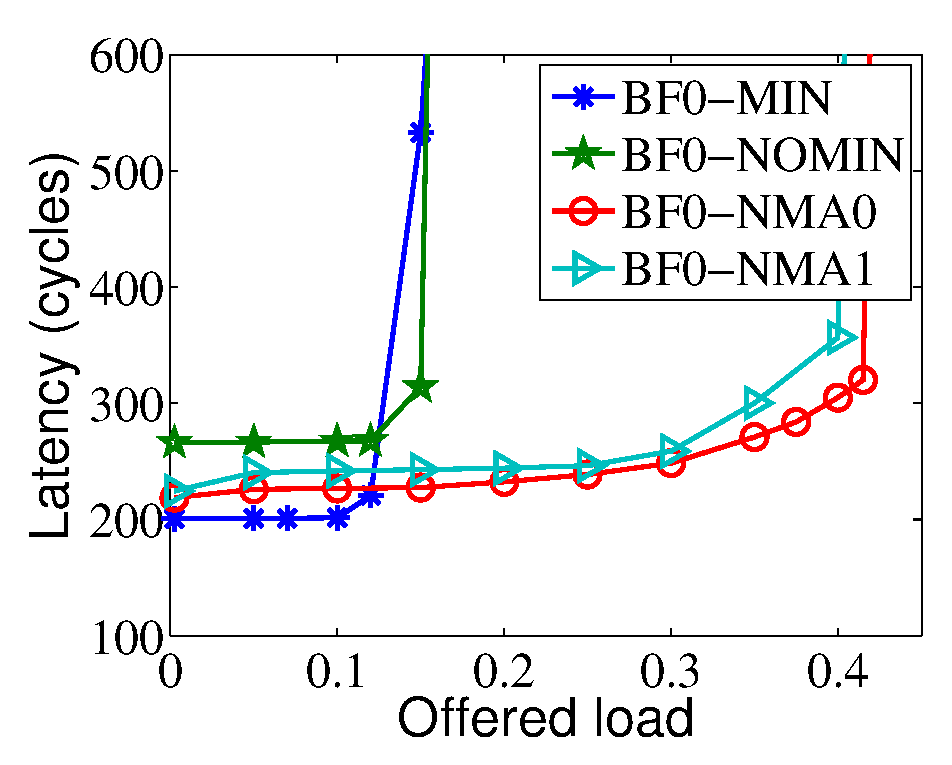
\includegraphics[width=.46\textwidth,height=.38\textwidth]{routing10Kadv0.eps}
  \label{raadv0}
  }
  \subfloat[BF1]{
    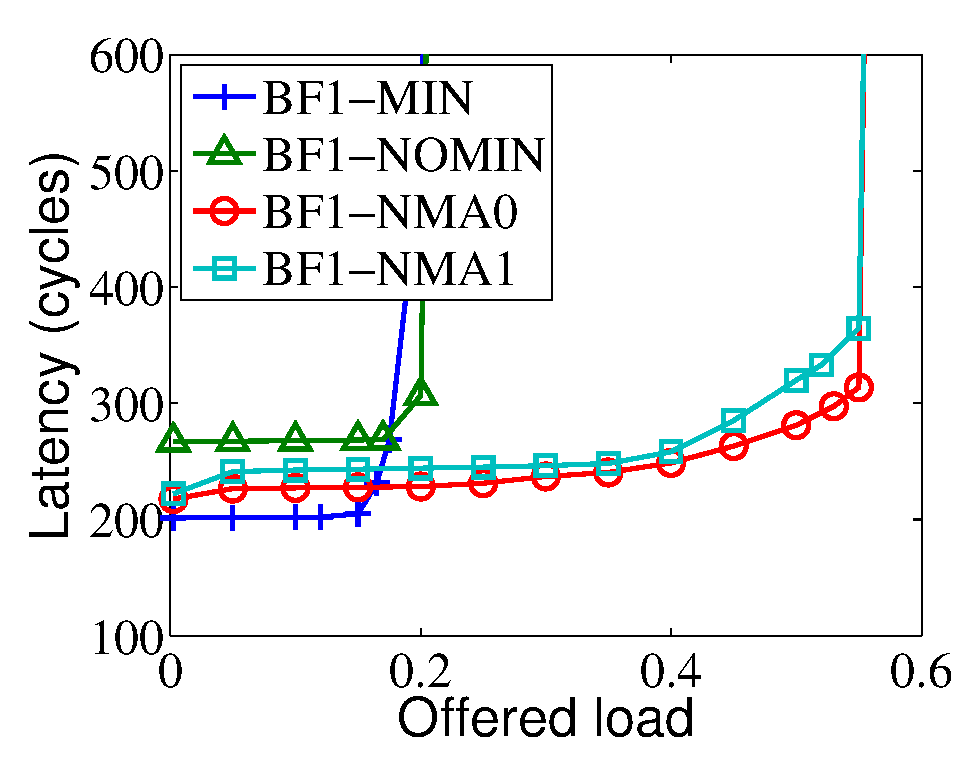
\includegraphics[width=.46\textwidth,height=.38\textwidth]{routing10Kadv1.eps}
    \label{raadv1}
  }
  \vspace{-.3cm}
  \caption{全局最差通信模式下不同路由算法性能}
  \label{l1ra02}
  \end{minipage}
  \end{figure}

  \subsection{不同的缓冲区大小和报文大小}

  我们也评测了在不同输入缓冲区大小和报文长度大小时BF的性能变化。
  图\ref{bufferpacket}和图\ref{bufferpacketadv}展示了采用物理布局
  链路传输延迟配置的拓扑结构在均衡随机通信模式下以及
  在全局最差通信模式下的性能结果。配置为512个切片大小的缓冲区和配置为256 个切片大小的缓冲区在均衡随机通信模式下的性能相近,因为缓冲区大小和链路延迟使得网络处于一个均衡的状态。但是在全局最差通信模式下,配置为512个切片大小缓冲区的性能比配置为256个切片大小缓冲区的性能略好是因为更多的缓冲
  区能够减少拥塞。在图\ref{bufferpacket1}和图\ref{bufferpacketadv1}中,报文长度越短延迟越低,因为长报文需要消耗更多的时间在路由器流水线上。


     \begin{figure}[t]
\setlength{\belowcaptionskip}{-.5cm}%
  \centering
 \begin{minipage}[t]{\textwidth}
   \centering
  \subfloat[Different buffer sizes]{
    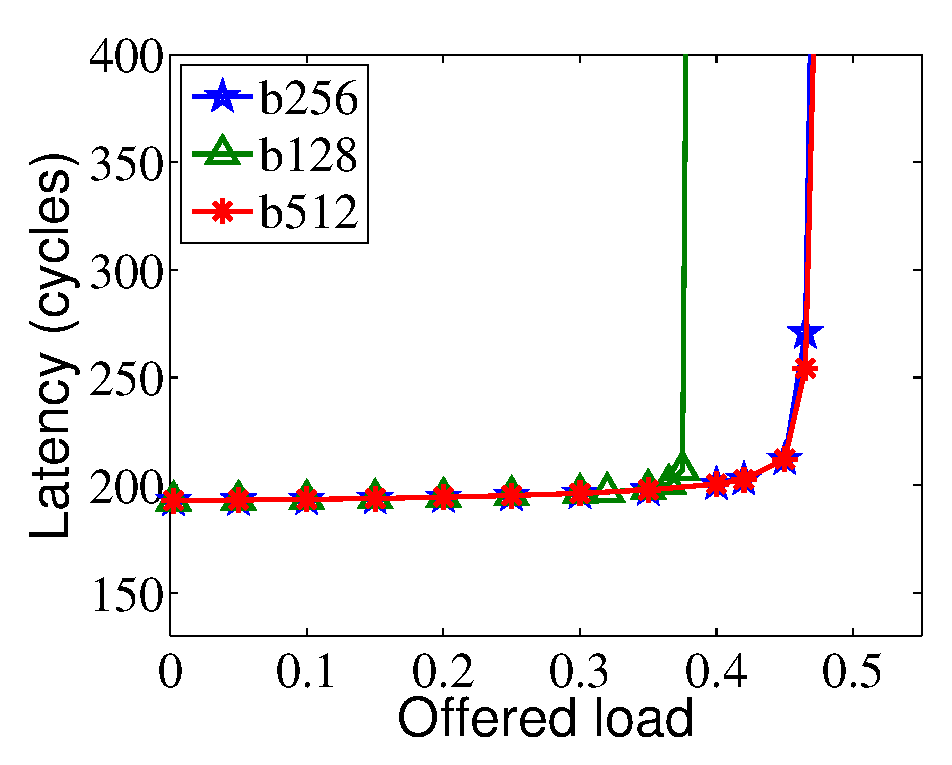
\includegraphics[width=.46\textwidth,height=.38\textwidth]{unbuf0.eps}
  \label{bufferpacket0}
  }
  \subfloat[Different packet sizes]{
   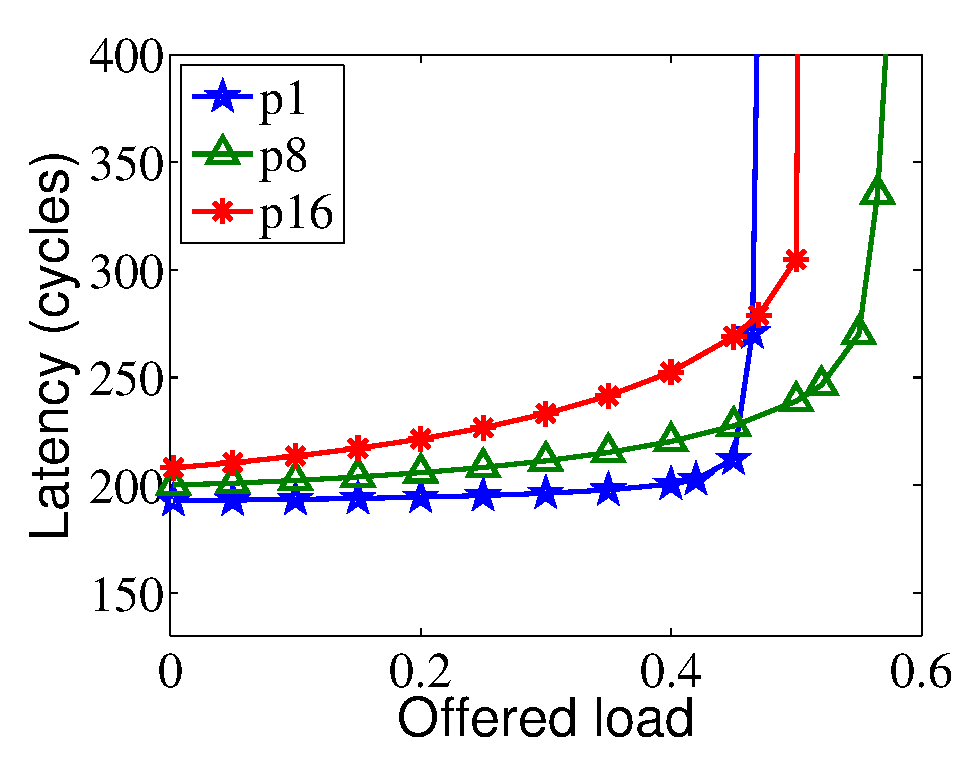
\includegraphics[width=.46\textwidth,height=.38\textwidth]{unbuf1.eps}
    \label{bufferpacket1}
  }
  \vspace{-.3cm}
  \caption{均衡通信模式下不同缓冲区长度和不同报文长度性能}
  \label{bufferpacket}
  \end{minipage}
  \end{figure}

 \begin{figure}[t]
\setlength{\belowcaptionskip}{-.5cm}%
  \centering
 \begin{minipage}[t]{\textwidth}
   \centering
  \subfloat[Different buffer sizes]{
    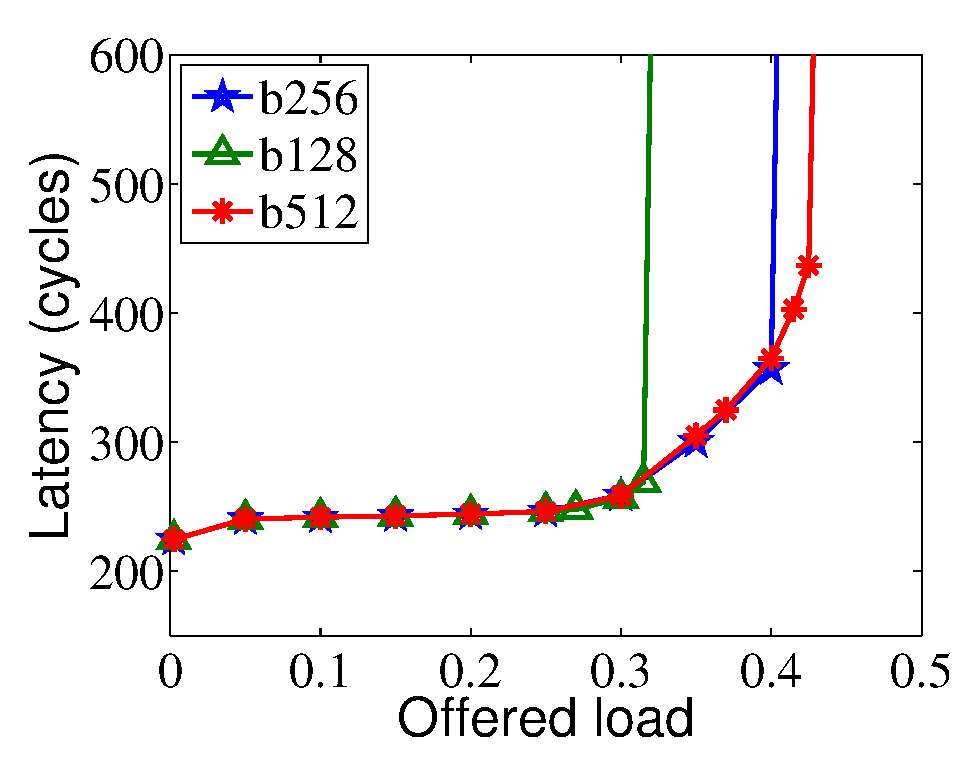
\includegraphics[width=.46\textwidth,height=.38\textwidth]{advbuf0.eps}
  \label{bufferpacketadv0}
  }
  \subfloat[Different packet sizes]{
   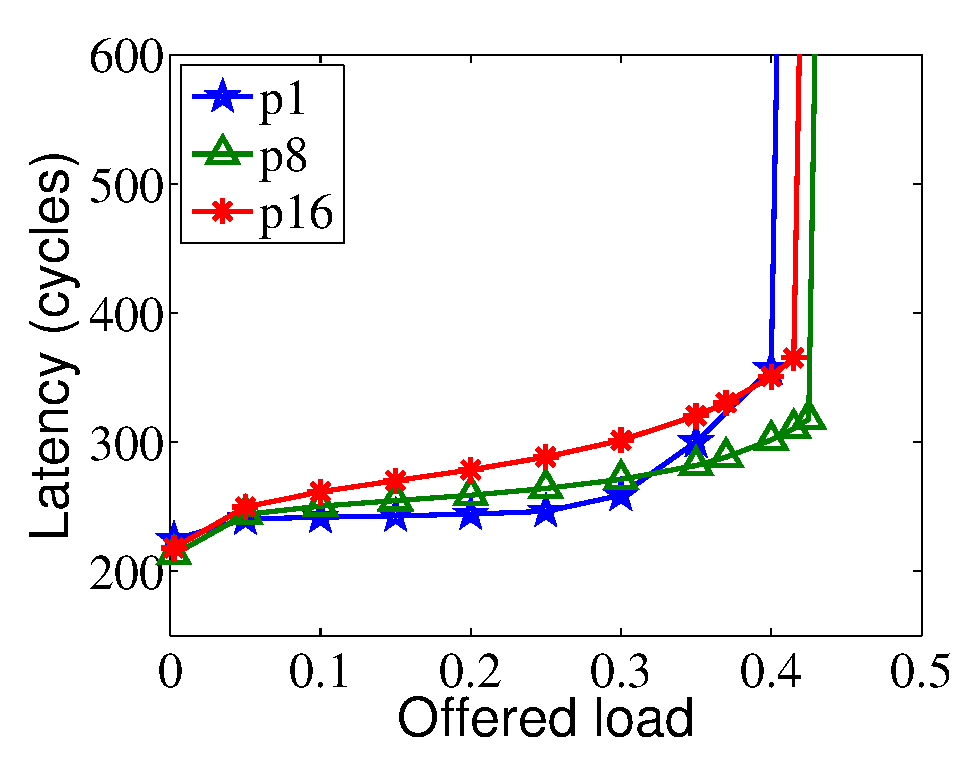
\includegraphics[width=.46\textwidth,height=.38\textwidth]{advbuf1.eps}
    \label{bufferpacketadv1}
  }
  \vspace{-.3cm}
  \caption{全局最差通信模式下不同缓冲区长度和不同报文长度性能}
  \label{bufferpacketadv}
  \end{minipage}
  \end{figure}

    \section{拓展与讨论}
   Bundlefly是基于MMS图和Paley图设计的多芯光纤友好的拓扑结构,不仅低
   延迟、多路径而且可扩展性好。

   \subsection{构造灵活的超级节点}

   超级节点内的拓扑结构可以灵活的使用Cayley图\upcite{MMS}来代替Paley图。
   Cayley图需要满足$a=4w_{1}+\delta_{1}$,其中$\delta_{1}\epsilon\{-1,0,1\}$。那么,我们构造的Bundlefly使用端口数为$k=\frac{3q-\delta}{2}+\frac{a-\delta_1}{2}+p$的路由器,其中端口数分配给其他路由器为$k'=\frac{3q-\delta}{2}+\frac{a-\delta_1}{2}$。在Cayley
   图中,a的取值范围比Paley图的取值范围大。实际上,MMS图中每一组的结构就是Cayley图而且Paley图是Cayley图的一种,其中$\delta_1=1$。因此,Cayley
   图满足Bundlefly结构的各项属性。

   \subsection{负载均衡路由算法}

   Bundlefly是一个多路径的拓扑结构。在一些节点对之间有多余一条的最短路径。我们需要设计一个负载均衡的路由算法去充分利用多路径来缓解网络的拥塞。
   而且,在最短路径路由的死锁避免策略下,使用$VC_0$的频率比使用$VC_1$的频
   率高。在大多数情况下,我们在没有死锁的情况下随机选择VC更利于VC均衡使用。例如,如果源路由器和目的路由器直接相连,我们可以使用$VC_0$或者$VC_1$来传递报文。

    \section{本章小结}

    随着互连网络规模的增加,通信带宽的需求也随之增加。板上集成光模块技术 的快速发展使得在系统构造中光纤的比重越来越大。多芯光纤将是一个新颖的、性价比高的方法来替代一捆单芯光纤来增加机柜间的带宽密度。它不仅
    能降低系统构造的复杂度还能提高系统可维护性。

    我们第一次提出一种大规模低直径多芯光纤友好的拓扑结构,Bundlefly。我们的目标不仅增加机柜间链路而且降低构造低直径E级系统对路由器端口数的要求。我们定义了一个优化问题即构造一个在给定节点度下更大网络规模且较小网络
    直径的结构。我们采用了multi-star product方法构造了一些直径为3的拓扑结构。
    其中,对MMS图和Paley图使用multi-star product方法的结构是最好的选择面不仅能保证较多的机柜间链路还能支持更大规模。

    Bundlefly是一个性价比高的直径为3的结构。不仅有多条机柜间链路而且存在
    多条最短路径。我们使用较少端口数的路由器构造同等规模的网络并能获得较高的供给比例。我们也设计了物力布局模型去分析不同拓扑结构和Bundlefly的性能。
    而且,Bundlefly因为有较多的机柜间链路在全局最差通信模式下展现了较好的性能。


